\protect\hypertarget{titlepage.xhtml}{}{}

\protect\hypertarget{index_split_000.html}{}{}

NO. 6 \textbar{} Atsuko Asano

Volume 2

\hypertarget{index_split_000.htmlux5cux23calibre_pb_0}{}

\protect\hypertarget{index_split_001.html}{}{}

\hypertarget{index_split_001.htmlux5cux23calibre_pb_0}{}

\hypertarget{index_split_001.htmlux5cux23calibre_toc_2}{%
\subsection{CHAPTER 1}\label{index_split_001.htmlux5cux23calibre_toc_2}}

\subsubsection{Of Life and Death}

\emph{Thou livest; report me and my cause aright}

\emph{To the unsatisfied.}

\emph{~ ~ ~ ~ ~- Hamlet, Act V Scene II~}

Shion closed the book. He could hear the sound of rain.

This underground room was cut off from most outside sounds. But for some
reason, the sounds of the wind and the rain always seemed to seep
through the walls.~

A mouse scurried up Shion's leg and perched on his knee. It twitched its
whiskers and rubbed its front paws together as if in request.

"You want me to read this book to you?"

Cheep.

"You really like tragedies, don't you. Why don't you pick something more
fun?"

The mouse looked up at him and blinked its grape-coloured eyes. Shion
adjusted himself in his chair and crossed his legs, with the mouse still
on his knee.

The chair had once been quite a fine piece of furniture. It was evident
from its sturdy build and the delicate patterns carved into the
chair-back. But now, it was worn and old; the colour was peeling in
various places, and the cushion had faded so much it was impossible to
tell what colour it had been before. Still, it was one of the few pieces
of furniture that this room had. A week ago, Shion had dug it out from
among the books that covered two-thirds of the room's floor space.

"There might be an even bigger treasure hidden in these books, if you
sorted them out." Shion had meant to sound serious, but Nezumi scoffed.

"Why don't you worry about building up some strength before thinking
about stupid stuff like that? You're a little boy who's probably never
had to do any physical labour since the day you were born. You're pale
and skinny enough as it is."

"I was in charge of cleaning duties at the park. I had to do physical
labour all the time."

Nezumi's shoulders hunched. His voice was tinged with contempt.

"Cleaning duties? Does cleaning count as physical labour in No. 6? All
you had to do was operate the robots that did the maintenance and
cleaning. What physical labour is, little boy―"

Nezumi grabbed Shion's arm and dug his fingers in so hard that he
winced. Nezumi's fingers, slender at first glance, had a surprisingly
strong grip.

"―is using these arms, your legs, and putting your back into it. Using
your own body. Remember that."

Nezumi's biting and sarcastic way of speaking didn't bother Shion much
anymore after he had gotten used to it. In its harshness and cynicism,
there was often a truth that he couldn't help but agree with, and
oftentimes he would come away more persuaded than offended. It was true,
the work that Shion did in the Holy City of No. 6 was just to tap the
keys of the control panel. He had never experienced the kind of labour
that made his own body creak under its burden. He had no experience of
what it was like to be damp with sweat, to have the skin of his hands
blister and tear, to have his muscles ache from exhaustion; to be
famished unbearably, and to fall into a comfortable slumber after a
day's work.

He had never experienced it once.

"That's why I'm going to do this," Shion said determinedly, pointing at
the mountains of books that piled high all over the room. "I'm going to
organize them, sort them out, and shelve them in order. If that's not
physical labour, I don't know what is."

"It'll take you a hundred years."

"I'll do it in a week."

Nezumi shrugged his shoulders again. "As you wish," he sighed.

"Do what you want. But stick with the books and bookshelves. Don't touch
anything else."

"You don't have much other than books and bookshelves in here."

"Like you said, you might find some amazing treasure. To tell you the
truth, even I don't know what's buried under these books."

The mice were chattering to each other from the nooks and tiny spaces
between the books. Shion picked up a small, light-green volume.

"Nezumi."

"Hm?"

"How long have you been living here?"

These bare concrete walls, thousands of books, this underground room― it
didn't seem well-suited to be a human dwelling.

"You didn't grow up here, did you? Where were you―"

He closed his mouth. He noticed that Nezumi's grey eyes were harbouring
a steely glint.

"I'm― I'm sorry."

Nezumi snatched the book out of Shion's hand and threw it aside.

"If you plan on staying here―" he wrapped his shoulders in the
superfibre cloth, and gave an impatient sigh. "Then do something about
that interrogation habit of yours. I don't know how much more I can take
of you nosing around every little part of my life."

"I'm not nosing around. I just wanted to know."

"Sniffing around and questioning people for every piece of information
you want is called nosing around. Remember that too."

Shion felt a jab of irritation at the way Nezumi's words seemed to push
him away. Indignation welled up inside him. He wasn't nosing around. He
grabbed Nezumi's arm as he made to leave the room.

"I barely know anything yet. That's why I wanted to know."

"And I'm saying that's called―"

"If it was something I could get by without knowing," Shion interrupted,
"I wouldn't want to know about it. But I do want to know. To me, this is
something I need to know. I want to know, and that's why―ach―" He bit
his tongue. He clamped a hand over his mouth and squatted on the floor
in pain. Tears stung at his eyes and the pain smarted in his mouth.
Nezumi burst out laughing.

"Geez, does clumsiness come naturally to you too? I never get tired of
looking at you. ―You alright?"

"Somewhat. Biting your tongue is really painful." When he had been in
No. 6 ― that was from when he was born, to the age of sixteen― Shion had
never once tripped over his words enough to bite his tongue. And it was
the first time, too, that he had grabbed someone's arm without thinking,
out of desire to say what his heart raced to tell, his words unable to
keep up with his thoughts.

"So?"

Nezumi knelt down, and peered into Shion's face. The light in his eyes,
which had the sheen of finely-woven cloth, had subsided to a gentle
glow.

"What do you want to know?"

"You―" Shion answered. "I want to know about you."

Nezumi's mouth fell open. He blinked several times.

"Shion, have you been reading any strange books lately?"

"Strange?"

"Like romance novels, the kind that are cliché and over the top. You
know, where a prince comes to rescue a damsel in distress, or when
lovers who are torn apart overcome trials and tribulations to reunite
again."

"I don't think I've read any of those."

"Then where the hell did you come up with that line? 'I want to know
about you'," Nezumi echoed in disbelief.

"I don't have to learn that from anywhere to say it."

"Are you serious about what you just said?"

"Of course. Nezumi―" Shion wiped his lips, and looked directly into his
grey eyes. "I want to know. I want to know because there are still so
many things I don't know. All I know about you is that you've saved me.
I don't know your real name, or how you grew up, or why you're living
here alone― or what you're thinking of now, or what you're planning to
do ― I have no idea. I don't know a single thing about you."

He was grabbed by the wrist. Nezumi's fingers were always cold, and
rigid.

"Then I'll tell you something. Put your hand here." Shion did as he was
told, and placed his hand on Nezumi's chest.

"What do you feel?"

"Feel―? Well, it feels like a man's chest, for one. It's hard, and
flat."

"I know, I know. Too bad for you, I don't have big breasts. What else?"

"Well..."

What did he feel on his palm through the rough fabric of Nezumi's shirt?
It was his heartbeat, his warmth, and the firmness of his flesh. Shion
hesitated to put it into words. He didn't know why. He withdrew his
hand, and curled his fingers over his palm. Nezumi chuckled quietly.

"My heart was beating, and it was warm. Right?"

"Of course. You're alive. It's normal for your heart to be beating and
for you to feel warm."

"It is. I'm alive, and I'm right here in front of you. That's all you
need to know. What more do you want?"

Nezumi stood up, and looked down at Shion. His gaze, like his fingers,
was cold.

"What you want is information," he said icily. "My birth date, my
development history, my height, weight, index of my intelligence, DNA
data. You just want information that you can convert into numbers.
That's the only way you ever try to understand other humans. That's why
you can't understand the living people that are standing right in front
of you."

Shion stood up as well. He clenched his fist harder.

"You're big on sarcasm, and love to make fun of people. You don't like
fish, and you're a restless sleeper."

There was a moment of silence.

"―Huh?"

Shion continued.

"You have an enormous amount of knowledge, and a wide range of it too―
but none of it is systematic. Sometimes you're fickle and
over-sensitive, but other times you're lazy and careless about the
details. You adore piping-hot soup, and you get really grumpy when it
doesn't have the right amount of salt. And last night, you kicked me
three times in your sleep."

"Hey Shion, wait a minute―"

"Since coming here, this is what I've learned about you. They're not
numbers. I would never substitute you for numbers. That's not what I
want to do."

Nezumi's gaze slid away from him.

"I'm just a stranger to you," he said. "You shouldn't be interested in
strangers. Four years ago, you saved my life, and I owe you a big debt
for that. So that's why, this time, I helped you out. So if you want,
you can stay here for as long as you wish and do what you want to do.
But never think of wanting to know more about another stranger."

"Why not?"

"Because it gets in the way."

"Gets in the way? Knowing things gets in my way?"

"Yes, for people like you. You're good at cramming knowledge, but you
give in easily to your emotions. You're quick to trust in people, and
try to attach yourself to them. I told you before, didn't I? Cut
yourself off, and throw away everything you don't need."

"Yeah, but...."

"But what you're doing right now is just the opposite. You're starting
to take interest in me and want to know more. You're trying to add even
more to your burden. You're hopelessly stupid, just hopeless."

Shion couldn't understand what Nezumi was saying. It was more
confounding and difficult to grasp than any scholarly book he had read.

"Nezumi, I don't understand what you're talking about." He voiced his
feelings truthfully. Nezumi shrugged slightly.

"The more you know, the more emotionally attached you'll get. Then we
can't be strangers anymore. And that'll be trouble for you."

"For me? Why?"

"When we become enemies, you won't be able to kill me." There was a hint
of a laugh in his voice. Shion dug his feet firmly into the worn carpet.

"While you're busy being caught up in your emotions, I can go ahead and
stab a knife into your heart. You know, a knife is a really ancient
weapon, but it can come in handy sometimes."

"Why do you and I have to become enemies? That's just absurd. That's
what's stupid, if anything."

"Really? I think it's pretty plausible."

"Nezumi!" Shion said heatedly.

There was a loud toppling noise as a pile of books fell over. A mouse
hopped onto Nezumi's shoulder.

"Well, if you're really gonna organize these books, you better get
cracking. One week will be over in no time. I'm going to work." Nezumi
turned nimbly on his heel and walked out the door. Shion felt all the
tension leave his body. He was cold and clammy. Conversations with
Nezumi sometimes made him so wrought with nerves that he broke out in a
cold sweat. Shion licked his dry lips.

"I don't even know what kind of job it is that you do," he muttered to
himself. "I only wanted to know. Who's the stupid one here?" He let his
words hang for a moment, then set out to organize the stacks of books.

"Shion." The door opened, and Nezumi's voice called him. A pair of work
gloves were tossed his way.

"You'll crack a nail if you use your bare hands." The door closed before
Shion could say thanks, and silence settled over the room again. This
casual act of kindness, or those cold, dispassionate words from a few
minutes ago― which one was he to believe? Shion couldn't grasp him. That
was why he wished could reach out and take firm hold. Shion pulled the
gloves over his hands, and lifted some books off the floor.

Of course. It's good to wear gloves when doing this kind of work. That's
another thing I didn't even know.

You just want information that you can convert into numbers. That's the
only way you ever try to understand other humans. The words that had
been slapped in his face minutes before still remained stubbornly in his
ears. This method of analyzing people through their data was something
Shion had learned all his life in No. 6, ever since he had been deemed
top-ranking in the Childrens' Examinations and was given a top-class
learning environment.

The human body is made up of 274 different types of cells, numbering 60
billion in total. He remembered perfectly the names, shapes, and
functions of each. He knew the locations and functions of each organ,
and had also learned about the transmission paths of signals between the
amygdala, perirhinal cortex and the hippocampus.

But it was no use to him. No matter how much he put his knowledge to
work, he was unable to understand the person with whom he'd been living
for almost a month.

Was Nezumi honestly thinking that they were going to become enemies some
day? That they would end up killing each other― was that possible?
Nezumi's words and actions were always shrouded in mystery, and confused
Shion greatly.

He couldn't grasp him. That was why he wished could reach out and take
firm hold. He wanted to know the part of Nezumi that couldn't be
substituted for numbers or symbols. Shion shook his head. The mice
scampered busily about his feet. I have to stop. Brooding over it isn't
gonna help. Right now, I have to wage war with these books.

He was soon damp with perspiration. His back ached, and his arms felt
heavy. But what interrupted Shion in his work was not in his bodily ache
or exhaustion, but in the pages of the books he went through. He would
casually flip to a story, and find himself sinking to the floor to read
the rest. Wholly engrossed, he would soon lose track of the hour. And
each time, a little mouse hopped up onto the page in stern reprimand.

"Give me one more minute. I'll put it away as soon as I'm finished
reading this part."

"Cheep cheep!"

"Alright, alright. I'm getting on it, okay? Are you satisfied now?"

And on the third day, he found it, under an old copy of a science
journal. A small, silver box. His emergency kit.

On that stormy night four years ago, Nezumi had appeared, sopping wet, a
sudden intruder in Shion's home. His shoulder stained with blood, the
dripping boy before him looked as if he was about to collapse. Shion had
extended his hand without thinking. His protective instinct had stirred
so strongly in him that he had even forgotten to feel fear toward the
intruder. Even after finding out that he was a VC― considered a violent
and dangerous criminal in No. 6― that feeling did not change. Shion took
Nezumi under his wing, and provided treatment for his wound and a
momentary respite. He didn't hesitate to. He couldn't help but do what
he did. As a result, Shion lost most of what he had, as well as a large
part of his secure and privileged life.

That night, Shion had treated the wound, painfully evident of the bullet
that had caused it, with the tools and medication in this emergency kit.
The next morning, there were four things missing in Shion's presence―
the red checkered shirt, the towel, the emergency kit, and Nezumi
himself. Of them, two were back in his hands. Or, rather, emergency kit
aside, perhaps it wasn't right to say that Nezumi had "come back" into
his hands. Shion was the one who had fallen into a trap, and was about
to be hauled to the Correctional Facility by the Security Bureau― Nezumi
was the one who had saved him, and brought him outside No. 6.

He wasn't the one that came back. I was the one that burst in and took
refuge here. That was the reality of it. He had fallen from the Utopian
City― even called Holy by some―into this underground room, where no
sunlight shone. He would probably never be able to return to No. 6
legitimately again. He had left his mother there. Was Karan still
thinking of him, even after he had been cast as an escaped criminal?
Shion knew it was fruitless to think about it, but his heart ached
nonetheless.

He couldn't throw it all away like Nezumi. He couldn't cut himself off.
He couldn't live without. He had to cling to something, else he would
crumble and fall. He had to have someone in his heart always, else he
would go insane.

Shion opened the lid of the box. It looked like the automatic sterilizer
was still functioning. A scalpel and a roll of gauze glowed dimly under
the faint reddish light of the sterile lamp. A nostalgic feeling welled
up in his chest as if he was meeting an old friend.

"Cheep-cheep! Chit-chit-chit!"

"What? I know, I know. I'm getting there. Geez, you're strict." Shion
laughed. As if in response, the mouse raised its front paws and
chittered.

* * *

By the time a week rolled around, Shion had managed to organize almost
all of the books that had been dominating most of the floor. Of course,
it was impossible to find shelf space for all of them, and many piles of
books still remained on the floor ― but it had cleared up a considerable
amount of living space.

"So what do you think?" Shion puffed out his chest proudly. Nezumi was
draped lazily over the chair. He yawned.

"The emergency kit, a couple blankets, a mug, and an old heater. Is that
all you managed to find?"

"That's a lot," Shion replied indignantly.

"Too bad you couldn't find an entry permit into No. 6."

Shion moved in front of Nezumi, and looked him directly in the eye. If
he was going to speak in earnest, he mustn't avert the other's gaze. It
was one of the things he had learned in his one month of living with
Nezumi. Shion bent over, and clasped each hand around the armrests of
the chair.

"What?"

Shion was now blocking Nezumi from the front. Nezumi shifted uneasily in
his seat.

"Nezumi, my mother is still in No. 6. She's my only blood relative. I
don't care how much you laugh at me for it, but I'll never be able to
cut her off. But― but let me say this. I have no attachments to life in
that city anymore. Even if someone told me I could go back in time, I
wouldn't want to go back to when I had the privilege to live in No. 6 as
its legitimate citizen. I'm serious― I wouldn't want to return one bit."

The grey eyes on the other end of Shion's gaze didn't blink once.

"You said that my life in No. 6 was fake. Now I've experienced it for
myself. And I never, ever want to return to a life that's fake, and only
peaceful and privileged in appearance."

"So you're prepared to live life outside of the Holy City, is that what
you're telling me?"

"Yeah."

"Do you know what kind of place this is?"

He hesitated to answer. Nezumi's lips twisted into a cold smile.

"You don't know anything," he said softly. "You don't know what it's
like to starve, to shiver in the cold, to groan from a wound that's
festered because it's been left untreated too long; you don't know the
suffering that follows when that wound becomes infested with maggots,
and you start rotting alive; you don't know how it feels to watch
someone die in front of you, while there's nothing you can do to help
them. You don't know a single thing. You're just rattling off pretty
words. You've experienced it for yourself, you say? You've only peeled
the surface of that city and sniffed at it, and already you're acting
like you know everything about it. It might be a city of lies, but in
No. 6 you have a warm bed, plenty of food and clean water. You have
fully-equipped medical facilities, recreational facilities, educational
institutions. Everything that residents here would never be able to
have, no matter how hard they wished. And you say you have no
attachments to those? That's arrogant of you. So arrogant it makes my
skin crawl. Either that, or you're a liar."

Shion drew a breath. He tightened his grip on the armrests.\\

"It might be arrogant― but I'm not lying. Regardless of what kind of
place is, I still want to continue living here. It's not because I got
chased out of No. 6 as a criminal. Even if I wasn't― no matter how
horrible this environment turns out to be, I want to stay here."

"What's your reason?" Nezumi shot back. "If you're not lying, and if
you're not trying to impress me with a model answer, what lead you to
make that decision?"

"I'm drawn to you."

"Huh?"

"You know things that I don't know. You've taught me things that no one
has ever taught me before. I can't say it well, but―" he hesitated. "I'm
drawn to you. A lot. That's why I want to stay here. I want to see what
you see, eat what you eat, and breathe the same air as you. I want to
hold in these hands what I would never have been able to get in No. 6."

Nezumi slowly blinked twice. Then, he placed a palm on his forehead and
shook his head slowly in exasperation.

"Shion, I've been noticing this for some time now, but―"

"Yeah?"

"Your language ability is worse than a chimpanzee."

"I've heard before that the genome of a human and chimpanzee are only
different by 1.23\%," said Shion, unfazed. "I don't think you should
mock chimpanzees."

"I'm mocking you. Idiot. Don't you have any idea what proper expressions
to use?"

"Was there something weird about what I said?"

"Don't use words like 'drawn to' so easily. It's a very weighty,
important word. You're only supposed to use it for a special,
irreplaceable person in your life."

"Then how am I supposed to say it? Do I say I love you?"

Nezumi heaved a long, exaggerated sigh. "Never mind," he muttered. "It
messes me up when I talk to you. Here," he pushed a thick book into
Shion's hands, and stood up. "Hamlet. Read it."

"I already have."

"Then read it again. Give that crippled language ability of yours some
good, hard training. Learn some words."

"Was I off-the-mark that badly?"

Nezumi's words quickened.

"You're just fascinated by new and unusual things. You're like a scholar
who's discovered a new planet, or a new kind of bacteria. You're just
itching with curiosity because you've met someone who's different from
all the people that used to surround you. That's it. You're not drawn to
me, and you're not in love with me. You're just excited about the exotic
animal you've discovered. Can't you even tell the difference?"

They were harsh words. They became sharp thorns that stabbed at Shion's
eardrums.

"I don't trust you," Nezumi said.

Shion raised his face, and his gaze collided with Nezumi's. He had been
biting his lip without thinking.

"I don't trust anything you say. You're someone who's been living in
artificial abundance since you were born. And you're arrogant enough to
be able to say you can throw away that fortune easily. ―Shion," he said
suddenly. "When you used to do that cleaning job at the park, you had to
do that ritual every morning, didn't you?"

The ritual was always the first task in Shion's work day. He had to lay
a palm on the image of the City Hall ― or Moondrop, informally ― that
was displayed on monitor of the maintenance system, and pledge his
allegiance.

"I hereon and ever pledge my unwavering allegiance to the City of No.
6."

"Our gratitude for your loyalty. Engage in your day's labour with
sincerity and pride as a good citizen of the City."

That was it. Every morning, he had repeated the same task. It had been a
sore discomfort for him. His youthful pride stung for having to repeat
these banal and grandiose words, and for this ritual itself, which
seemed foolish.

Nezumi gave a short laugh.

"You hated it, didn't you."

"Yeah."

"Felt suffocated, didn't you, being forced to declare your loyalty."

"Yeah... now that you mention it."

"But you put up with it," Nezumi said. "Instead of retaliating, you
recited this pledge every morning, not meaning a single word of it, and
pretended it didn't bother you. Let me tell you something, Shion: words
aren't things that you can toss around casually. You can't let yourself
be forced to say something, and just put up with it. But you don't know
that. So that's why I'm not going to trust you."

Nezumi's hand suddenly extended toward him. His palm touched Shion's
cheek.

"Did that hurt?" he asked gently.

"Quite a bit."

"―I don't have any grudge against you. And I don't hate you, either."

"I know..." Shion answered quietly. "That much I can tell."

"Shion."

"Hm?"

"Feel like going outside?"

His fingers caressed Shion's hair.

"You're fully recovered, now, aren't you? Feel like seeing for yourself
the place you've decided to continue living in?"

Nezumi's hand slowly drew away. Several strands of white hair clung to
his long fingers. Shion's hair still had some lustre despite being
drained of its colour, and to certain eyes he figured it might look
pretty. But he felt its beauty to be cruel. In a single night, the
colour had faded from his hair, and he had been scarred with a red band
that slithered like a serpent over his entire body. He had been seen by
children, who had shrieked at the sight of him. He couldn't forget the
look in their eyes. They were filled with dismay and horror like the
eyes of one who beheld a deformed monster. But he had to go outside. He
wanted to see the world he was going to live in with his own eyes, hear
the sounds with his own ears, smell with his nose, and feel it on his
own skin. Then, maybe, he would speak to Nezumi about it again.

No matter what kind of place this is, I want to keep living here. Rather
than being surrounded by falsities, and being forced to swallow banal
words, I want to live here― even if it means I have to struggle―

"We can dye your hair, if it'll make you feel better at all," Nezumi
said. "Black, brown, green― whatever colour you wish. What do you wanna
do?"

"No, it's fine."

"You're going to keep it?"

"Yeah, I'll keep my hair like this. White hair isn't so bad. I figure
it's better than being completely bald."

Nezumi lowered his face. His shoulders were trembling.

"You're really funny, you know that?" he said, his voice shaking from
holding back a laugh. "Seriously. I mean, really."

"Am I?" said Shion dubiously. "No one's ever really told me I'm
funny..."

"You're a natural comedian. You should toss the theory books and study
comedy instead."

"I'll think about it."

"You should. Right― tomorrow, then, I'll show you around."

"Alright," Shion agreed.

"And there's one place you definitely need to go to."

"Latch Building," Shion answered for him.


\includegraphics{Images/memo1.png}\\

It was a memo from Karan, and it was a cryptic one― Shion didn't know
where it pointed to, or who was going to be there.

"Did you find out where Latch Building is?"

"Nope," Nezumi replied. "We don't have any fancy numberings for our
buildings here. But once upon a time this place used to be a decent
town, and I was able to get a map from then. And there's a region that's
marked LK-3000."

"You looked all of this up..." Shion murmured in awe.

"Just to kill some time."

"I didn't think you had time to kill. You always seem so busy―"

"Oh, and write a letter," Nezumi interrupted nonchalantly.

"Huh?"

"To your Mama. But keep it within 15 words. Just a simple note. The
mouse here says he misses your mother's homemade bread."

"You'll deliver the letter for me?"

"More like a memo," he said brusquely. "Under 15 words. I can't
guarantee it'll get there safely."

"Nezumi."

"What?"

"Thank you."

Nezumi shrank away from Shion and fixed him with an appalled stare.

"Please, can you not look at me like that? It gives me the willies.
What'll happen tomorrow will happen tomorrow. I'm gonna take a shower.
Oh, and before you write a letter to your mama, read the poor little guy
a story. He's been waiting all this time."

Nezumi disappeared into the bathroom. Shion curled up in a chair, and
opened the book he had been passed earlier. There was a faint whiff of
the smell of paper. He was drawn in instantly, and soon lost himself in
its pages.

\emph{If thou didst ever hold me in thy heart,}

\emph{Absent thee from felicity awhile,}

\emph{And in this harsh world draw thy breath in pain}

\emph{To tell my story.}

Hamlet drew his last breath in the arms of his friend. Shion slowly
closed the book. There was the sound of rain. He wondered why it always
seemed to seep through the walls into this underground room. It seeped
through and reverberated, like the soft sound of music.

And in this harsh world, draw thy breath in pain― maybe that's what
living on in this world meant― to suffer in pain. And Nezumi knew this.
It had been ingrained into his body. A mouse chirruped at his foot.

"Oh, sorry about that. Which one do you want me to read?"

The mouse climbed up onto his knee, and rubbed its front paws together.

"You want me to read this book to you?"

Cheep.

"You really like tragedies, don't you. Why don't you pick something more
fun?"

He crossed his legs, with the mouse still perched on his knee.

"Read him the tragedy," Nezumi's voice spoke from behind him. He hadn't
even noticed Nezumi coming out of the bathroom. He hadn't heard a sound
or felt any presence.

"You have a good voice. This little guy loves to be read to. And he
loves to listen to you read tragedies."

"Really?"

The mouse blinked its grape-coloured eyes at him. Shion guessed it was
his way of saying yes.

"Okay, okay. Then from the top of Act Five―"

"Shh―" Nezumi's damp hand pressed over Shion's mouth. "I hear
something."

"Huh?"

Before Shion could ask what it was, it reached his own ears. The sound
of footsteps clambering down the steps. The heavy door was being banged.
Someone was knocking on the centre of the~

door, and its sound was frantic, though not altogether strong.

A child.

A child was knocking desperately on the door. Shion stood up, and made
for the entrance.

"Not so fast." Nezumi stopped him. Under his wet bangs, his grey eyes
beheld the door warily.

"Don't open the door yet."

"Why not?"

"It's dangerous. Don't open the door without any defense."

"It's a child knocking. And it's urgent. Something must have happened."

"How can you be so sure? An armed soldier can knock on the bottom half
of the door, no problem."

Shion's gaze travelled from Nezumi's face to the door.

Help me.

He thought he heard a weak voice cry out in plea. He swallowed. He
unlatched the door, and gripped the handle.

"Shion!"

He opened the door. A cold draft blew into the room. It was getting dark
outside, and a chill wind was blowing.

A girl was standing in the gathering dark. Her eyes were filled with
tears as she looked up at Shion. He had seen her before. She lived in
the barracks in the hollow under the slope. She was the girl he had not
been able to forget― the girl who had shrieked at Shion's whitened hair
and red scar that snaked up his neck. For the first time, in this gaze,
he had been beheld like a deformity. But now, her large eyes were
brimming with tears, and contained no hint of terror. Instead, they were
bright with frantic urgency.~

"Help me― please― he's dying."

Shion swiftly took the girl by her hand, and began to clamber up the
stairs. He hastily yelled over his shoulder.

"Nezumi, bring the emergency kit, and some blankets!"

Then he burst outside, into the wood of bare branches and fallen leaves.

\hypertarget{index_split_001.htmlux5cux23calibre_pb_21}{}

\protect\hypertarget{index_split_021.html}{}{}

\hypertarget{index_split_021.htmlux5cux23calibre_pb_0}{}

\hypertarget{index_split_021.htmlux5cux23calibre_toc_3}{%
\subsection{CHAPTER 2}\label{index_split_021.htmlux5cux23calibre_toc_3}}

\subsubsection{The Place of the Gods}

\emph{Then the goddess Hannahanna decided to use her last resort. She
gathered not several, but hundreds, thousands of bees, and said, "You
are small and nimble, and fly as swift as the light, so you shall surely
be able to find the god Telepinu. Now, go."~}

\emph{~ ~ ~ ~ ~- The Disappearance of Telipinu, Hittite Myth}

There was a person collapsed at the foot of a spindly tree whose bark
was whiter than the rest. He was a little boy, even smaller than the
girl in size. He was writhing in pain. Shion took him in his arms and
sat him up. Even in the settling dusk, he could tell that the boy was
deathly pale. He was clawing at his throat, and his mouth was open, but
his lips were bloodless.

Suffocation. He was choking from something stuck in his throat. There
was no time to waste. Supporting the boy's belly with one arm, Shion
thumped his back with the palm of his other hand.

"Spit it out. Come on," he urged. Twice, then a third time, he kept
hitting the boy's bony back. Four times, five times...

The boy wretched, and vomit spilled out of his mouth. There was a dark,
round object mixed in with it. The boy twitched slightly.

"Water! Bring water!" Shion commanded Nezumi again. He lay the boy down,
and brought his own cheek to the boy's mouth. He could feel definite
breathing. He's alright, he's breathing. He didn't need to clear the
boy's airway, or give him artificial resuscitation. But his
consciousness―

"Call his name."

The girl responded quickly to Shion's words. She bent over the boy,
bringing her face close to his, and called his name.

"Rico, can you hear me? Rico."

"Rico, can you breathe?" Shion called after her.

The boy's chest swelled largely. His eyelids fluttered and opened. A
tear spilled over and rolled down his cheek.

"―Sis―"

"Rico!" Shion gently restrained the girl as she tried to throw her arms
around the boy. He slowly raised Rico's upper body off the ground, and
brought a cup of water to his mouth.

"Can you drink this?"

"Yeah."

"Good boy. Drink it slowly. So your name is Rico, huh?"

"Yeah."

"Rico, can you hear your sister's voice and my voice clearly? Can you
see us just fine?"

"Yeah― and the water tastes good."

"You're a good boy," Shion enthused. "You've done a really great job.
Does your stomach feel alright? Does your chest hurt at all?"

"My throat..."

"Hm?"

"My throat hurts..."

Rico had probably torn at his throat in pain, for it was covered in
scratches which were beginning to bleed. Shion retrieved some gauze and
rubbing alcohol from the emergency kit. They were four years old, but
now, this was all they had.

"This is going to sting. Don't cry."

"I won't."

He swabbed the wounds, pressed a fresh piece of gauze to them, and
wrapped Rico's neck with a bandage. Shion could only give him the most
basic of emergency procedures. This was the best he could do. If he had
said anything along the lines of 'to the hospital', Nezumi would have
laughed in his face. Shion knew very well that in this area, the West
Block of No. 6, there was no such thing as a decent medical facility.
From what Rico had vomited out, Shion picked out what appeared to have
been blocking his airway.

"A nut?" It was small and round. "Why would this be―"

Rico hung his head. Nezumi folded his arms as he stood, and gave a short
sigh.

"He was hungry."

"Huh?"

"He was probably so hungry he couldn't bear it anymore. That nut― if you
grind it into flour, it's― well, it's edible. He was probably in the
middle of gathering them when he got hungry. He got so hungry he decided
to put one in his mouth, which was all good until he swallowed it by
mistake― is my guess of what probably happened."

"Rico's always hungry," the girl said. "Even if Mum gives him part of
her bread, he's still hungry."

"It's such a tiny piece of bread," Rico protested. "One bite, and it's
all gone." He dissolved into a fit of coughs. His voice was raspy, and
his face was still pale. Shion wrapped his body in a blanket.

"Keep warm. If your neck still hurts, I'll treat it for you. Come again
anytime."

"Take them home."

Shion raised his face at Nezumi's words.

"Me?"

"Yeah, you. You helped them, so finish your job and see them through.
They live in the house down this slope, it's not too far. Their mother
is probably getting worried right about now."

That meant he would have to show himself to an adult. Shion stood up. He
didn't know why, but he had started to shake.

"But I―"

"You'll have to go out there one day anyway. If you're getting scared
now, you'll never be able to walk the streets. ―Well, not that it's any
of my business. But if we stay out here in the rain any longer,
someone's going to catch pneumonia."

He had forgotten that it was raining. Shion finally noticed its
coldness. It seeped right into his bones, and reminded him that winter
was approaching.

"Well, I'm off. The prince can do as he pleases." Nezumi turned his back
to them and descended down the steps below. Rico sneezed. The girl
extended her small hand and grasped Shion's fingers.

"Thank you."

"Huh?"

"Thanks for saving my little brother."

"Oh― no, I― It's not―" Shion stammered. "You don't have to thank me.
What's your name?"

"Karan."

"Karan? That's the same name as my mother."

"Really?"

"Yeah."

The girl smiled. Shion could feel the warmth of the girl's hand as she
clasped his fingertips. He scooped Rico up, blankets and all.

"I'll take you two home. Kalan, lead the way."

There was steam rising out of the pot on the kerosene heater. Inside it
was soup. As he stirred the broth of vegetables and meat, Nezumi gave a
sigh. He flinched when he realized he had sighed without thinking. A few
droplets of soup splashed out of the pot, and hissed as they hit the RDF
heater.

He hated sighing. Sighing on purpose was a different matter― but this
kind of sighing, the kind that escaped his lips without his knowing,
irritated him.

"Never sigh in earnest. Never cry. You'll be taken advantage of by
demons." He had been told that by an old woman, so far in her years that
age seemed not to matter. "Sighing creates an opening, a vulnerability.
If you want to stay live, keep your mouth shut. Never let anyone see
your weak spot. Let your heart warm to no one. Never trust anyone but
yourself."

They were her dying words. She had been shot through the chest and was
frothing bloodily at the mouth, but her words had rung clearly in his
ears. Nezumi didn't think of ever forgetting them. Even if he did, her
voice would not let him. It clung tenaciously to his mind, and refused
to let go.

But he had turned his back on it. He had let an unheeded sigh escape his
lips without even realizing. All thanks to him. He tsked his tongue in
frustration.

Maybe it was a mistake to bring Shion here. He seriously thought so.
Shion had opened the door without hesitation. He had thrown it open
wide, without even checking what was on the other side, or concealing
himself in shadow. If they had been unlucky, he would have lost his
life. Even if the visitor had not been an armed soldier, it may as well
have been an armed robber using a child as bait. Here in the West Block,
it would not be an uncommon thing. But that was something Shion didn't
know. He didn't know how to be suspicious or cautious, or to be afraid.
It was the ignorance and recklessness of one who had grown up in safety
and security.

He honestly felt that he had taken a dangerous and troublesome burden
under his wing. No one had forced him to. He had born the burden of his
own will, because he wanted to return the favour he owed. There was no
way he could have let him die ― Shion, who had saved his life, expecting
nothing in return.

There was no way of returning a favour to the dead, and Nezumi didn't
want to carry a debt that he would never be able to repay. That was why
he rescued and brought Shion here. But now he thought it may have been
careless for him to do so. Maybe he had brought with him a bigger risk
than he had imagined. An oblivious and careless, dangerous and
troublesome―

He threw a glance at the door.

But if Shion had not opened the door that time, Rico would not have been
saved. It didn't take a lot of time for a choking young child to lose
his life. Swift action and appropriate treatment ― thanks to that,
Nezumi hadn't had to see a small body with its face permanently
contorted in pain. A life had been saved. It was the same as the stormy
night four years before. That time, it was him― this time, it was Rico.
Shion, both times, had taken them in recklessly and as a result, saved
them.

Shion knew the world only through theorems and rationales. He was naive
and hadn't even learned how to doubt the trustworthiness of others. He
was naturally oblivious, he was clueless, idiotic, and didn't even know
who Hamlet was. But Shion was also definitely above him in some ways.
Not in knowledge or skill, but ― but what?

"I'm drawn to you."

Was it the power to attempt at this embarrassing confession, and to
believe that his sincere feelings would actually get across? Was it the
power to lend a hand to a total stranger without thinking of the risk it
reflected on himself?

He didn't know. All he knew was that Shion was, indeed, dangerous and
troublesome. He was very― there were footsteps. Knocking. The door
opened soon afterwards. Shion had come home.

"If you're gonna knock, wait for an answer before opening the door,"
Nezumi said curtly.

"Not like you would answer anyway, right?" replied Shion lightly. "But I
noticed you left the door unlocked for me."

"Huh?"

"The lock. I thought you'd lock the door, but you kept it open."

He was right. He hadn't locked the door. How reckless of him.

"Look at me, I've fallen under your horrible influence," Nezumi said
woefully.

"What's that? ―Hey, look, I got some grapes as a thank-you gift."

The grapes were small and the whole bunch was rather pitiful.

"She offered me dried fish too, but I told her no thanks."

"Oh?" said Nezumi sardonically. "So even you felt bad about receiving
handouts from the poor."

"No. It was because you don't like fish."

"Me? I'll eat fish. I'm not fortunate enough to be picky about my food."

"But you told me once you didn't like it much."

"What I said was that I can't eat raw fish. Meaning, this place is way
too unhygienic to even think about eating fish raw."

Shion blinked, and put a hand to his hair.

"Oh. Oh well. ―But I'm glad, though."

"About what?"

"Kalan's family― oh, Kalan is the girl's name, by the way―"

"I know."

"Oh, you knew? It's the same name as my mother's."

"Your mother's name isn't any of my concern, but.... So? Did it bring
back memories of your Mama and bring you to tears? Poor thing."

He had meant it as a sarcastic remark, but Shion shook his head gravely.

"No, that's not it. There was another child there, a girl, younger than
Rico. I think that fish was supposed to be their supper. One dried fish,
for the three of them. It would have been alright not to accept that,
right? But their mother insisted that I accept the grapes. She was
really grateful. It kind of made me happy."

"You really think so?"

"Huh?"

"If that kid had died, there would be more to eat for Kalan and the
other girl. Even for Rico― wouldn't you have thought it would be better
for him to die rather than grow up in constant hunger? Maybe you haven't
actually done them a favour at all."

Shion sat down in front of the heater. His white hair, leaning more on
transparent, was tinged red with the colours of the flame. His youthful
hair had lost its colour, but still retained its shine. It's beautiful,
Nezumi thought.

Shion's head of hair glimmered as it reflected the light of the things
around it, and Nezumi extended his fingertips to touch it. His hair felt
slightly coarse, but ran through Nezumi's fingers easily. It felt like
ordinary hair, no more, no less.

"You told me to live," Shion said quietly, his face still turned to the
flames. "Nezumi― you said there's meaning to being alive, and that's why
I should live. That's what you said."

"I just said whoever lives wins."

"That's the same thing, isn't it?"

"How should I know?"

The dead could not speak. All they could do was lay there as a corpse,
and return to the earth from which they came. They had no way to speak
of the hatred, the cruelties, anguish, loathing or grief they went
through. That was why he had to live. He would live, preserving
everything in his memory, and pass it on.

No. 6.~

It was like an artificial flower that left no seeds behind. It bloomed
on the blood and corpses of a countless number. I'll pull you right out
of the ground one day. Then you'll have no choice but to hear the voices
of the dead, their hatred, their hardship, their anguish, their
loathing, as it wells up out of the very ground and soaks the earth.
I'll make sure you hear, even if you plug your ears. Until then, I'll
live and remember. To forget is not a choice. His own self didn't allow
him to.

"I got complimented." Shion looked up at Nezumi, and grinned.

"Complimented? For what?"

"My hair. Kalan's mother said it was nice. She said it was really
unique, and really pretty."

Nezumi shrugged.

"Well, it's unique, for sure. There are tons of kids around here that
have white hair from malnutrition, but no one with a whole head of snowy
hair like you."

"She didn't just say it was unique. She said it was pretty."

"Are you gushing about how someone complimented your hair? What are you,
a girl?"

"But― well, you know, it gives me a bit of confidence," said Shion
happily. "For when you show me around town tomorrow."

"Who said I was going to show you around?"

"You said so."

He did say so. He had said that he was going to show Shion around.
Nezumi felt like a sullen child. He averted his gaze from Shion.

"I'm going to go about my own business. You go about yours."

"Okay. I'll mind my own business and tag along. Oh, and one more thing―"

"What now?"

"I promised Kalan and Rico I'd read to them when I have time. I found a
lot of picture books in your stash, so―"

"You're gonna read to them here?"

"If it's sunny, I can take them outside."

Nezumi came close to sighing again, but he caught himself in time to
seal his lips and hold it in.

"Are you trying to make this place a kindergarten?"

"Are there that many children around here?"

"Oh yeah, tons. But this is my place. Don't go around doing things
without my permission, and don't think you're entitled to everything."

His words turned crude. There was a stinging irritation within his
chest. Being with Shion irritated him. He felt like his restraint would
snap any minute. It wasn't because Shion was being reckless or imposing,
he admitted that Shion wasn't― it was because he couldn't see through
him. There was no way to predict what Shion was thinking or what he
would do. His actions and words always seemed to hit Nezumi out of the
blue. It was tiring.

Shion was setting plates out on the table. The soup was finished, and
its gentle aroma filled the room.

"I wasn't thinking I was entitled to anything― it's just that, since
Kalan, Rico and I are friends now―"

"Huh?"

"Friends," Shion repeated. "They're the first friends I've made since
coming here. Well, not that I had many friends back in No. 6," he added
as an afterthought. "I think Safu was the only one."

"She said she wanted to sleep with you. You don't call that 'friends'."

He remembered the ends of her short hair that draped prettily on the
back of her neck.

Shion, I want to have sex with you.

She had put her all into this confession, and Shion had not been able to
handle it. What a guy you've fallen for, huh, he remarked in his mind to
the girl he barely knew. For some reason, he was suddenly overcome with
the urge to laugh.

"What?"

Shion cocked his head to the side. Two mice sitting atop a pile of books
tilted their heads too, as if to imitate him. Nezumi burst out laughing.
He squatted to the ground, and gave in fully to the wave of mirth that
bubbled up inside him.

The rain let up before noon but the clouds still lingered, and the
ground remained cold as dusk approached. Nezumi was walking briskly
through the throng. Shion was doing his best to keep up behind him. He
was out of breath. He was jostled, bumped, and yelled at; he felt the
gaze of countless curious eyes raining down on his head; the smell of a
dozen things reached his nose, so mingled and melded into each other
that he couldn't tell what they originally were; the muddy ground
tripped up his feet; a sprawl of barracks and tents lined the road, and
from them, thick smoke billowed rudely into the passerby; in the air,
angry bellows, seductive coos, and merchants' cries clashed clamorously.
He felt dizzy.

The older district of Lost Town, which was where he took up residence
after being forced from Chronos, was also bustling and lively. But
compared to what he was seeing now, it seemed like a tranquil getaway.

In No. 6, there were designated roads and paths for both people and
vehicles going in each direction, and as a fundamental rule, stopping
suddenly or going the opposite way was prohibited. Everyone walked in
the same direction, in the same orderly fashion. It was rare to ever
bump into anyone, or be stopped by an acquaintance. Nothing occurred
suddenly or unexpectedly. Everything was managed to prevent such things
from occurring. No. 6 was that kind of place.

A roar of voices suddenly erupted close by. Shion was shoved violently
aside. He lost his footing, and fell forward onto his knees in the mud.
Several men thundered past him. Something fell from one of their arms,
rolled, and came to a stop in front of Shion. It was an orange.

"Thief!"

A man burst out of one of the shops in the barracks, holding a gun. He
was towering, and very fat.

"Them thieves!" he roared. "Someone catch 'em!"

No one moved. Some smirked as they looked on, others showed no interest
at all, others were shouting unintelligibly; and all the while, the
so-called thieves were retreating further away into the crowd.

Shion's breath caught in his throat. The gigantic man was taking aim
with his gun. Passers-by who saw him squatted hastily to the ground to
take cover.

Is he nuts? Shion couldn't imagine this man being in his right mind to
open fire into this crowd of people. But the man's face was set in
determination. The long muzzle of his outdated firearm was pointed
straight before him. The fleeing men bumped into an old woman and pushed
her aside as they continued running. She yammered something at them,
then returned to hobbling down the centre of the road. She was oblivious
to the gun that was pointed her way. The giant's thick finger wrapped
around the trigger.

Shion threw himself at the man just before his hairy knuckle jerked to
fire the gun. With as much strength as he could muster, he knocked the
muzzle of the gun upwards.

He felt a heavy impact slam his hand, and a shot blasted in his
eardrums. The muzzle of the gun spewed fire into the darkening sky.
Shion staggered. His feet were swept from under him, and he was slammed
to the ground. His breath died on his lips.

"The hell do you think yer doin'?"

The man towered over him with his gun raised, filling every inch of his
vision. Shion rolled quickly to the side. The giant moved nimbly for his
appearance, and Shion was met with a firm kick in the ribs.

Shion grunted in pain. He couldn't speak. His stomach lurched.

"One of their little friends, eh?" the giant snarled. "Little fucker,
takin' a swipe at my merchandise."

The man's boot gave off a greasy, animal smell. And it was swinging
straight toward his stomach again.

"I'm not one of them!" Shion screamed, barely dodging the blow. I have
to scream, or else he'll really kick me to death. There was no hint of
hesitation in the blows that showered down upon him.

"I'm not― I'm not one of them," Shion persisted.

"Shut up!" the giant bellowed. "Now those bastard thieves 're gone.
Thanks to yer gettin' in the way."

"If I didn't intervene, someone could have been killed," Shion
protested. "Opening fire in a place like this ― what if you'd hit
someone?"

To his astonishment, the man started laughing. Laughter rose from the
crowd that lined the streets as well.

"And so what if I did?" the man roared, emanating his beastly odour.
"What's that got to do with me, eh?" His expression suddenly darkened,
and he roughly grabbed Shion by his hair. "You and yer strange mop o'
yers. I don't like the looks o' you."

He was pulled to the ground forcefully. His scalp burned with pain, and
it felt like it was being torn off. But even stronger than the aches on
his body were the feelings of wrath and humiliation that seethed within
him.

"Stop it!" Shion yelled.

Stop it. Let go of me. How dare you treat me like cattle.

Shion threw himself at the man again, and slammed his body into him as
hard as he could. He felt his elbow dig firmly into the man's swollen
gut. The man let out a muffled groan and fell on his knees. The crowd
had formed a ring around them. Clapping, whistling and raucous laughter
erupted periodically.

"That's the spirit, young'un. Give 'im what he deserves!"

"Kill 'im off, ol' man! There's no use wastin' time here!"

No one tried to stop them. Everyone was enjoying the spectacle from a
safe distance. Shion searched the jeering crowd for a pair of grey eyes.
He couldn't find them.

"You little―"

He heard a booming roar that sounded more animal than human. Then he
felt a blow bludgeon his cheek. Sparks burst before his eyes, and his
vision went dark for a short instant. Something warm was filling his
mouth. Unable to bear it, he spat it out. Saliva mixed with blood
splattered and oozed over the dirt.

"Playin' funny tricks!" The man's face was flushed red, and he was
shaking in rage. His eyes were bloodshot, and his veins were raised and
throbbing over his skin like a crimson web. The murderous intent that
radiated from him was unmistakable.

"Yer gonna pay for this," he growled. The gun was aimed right between
Shion's eyes. Shion couldn't close his gaping mouth. He felt like his
heart was going to burst out of his chest. And still, no one stopped
him. In this crowd of people that surrounded them, not a single one
stepped in to stop the man. He felt nauseous. He couldn't tell whether
the muzzle before his eyes was real or just an illusion.

"Hey," a deep voice punctuated the din. It belonged to a man who was
roasting meat at the front of his store. Pieces of blackened meat
covered the grill, which was billowing thick, sooty smoke. "Don't be
makin' a mess in front of my store," he said.

"I en't makin' a mess," the man growled.

"You were 'bout to, you were. If you go blowin' brains and blood all
over the place, everyone's gonna lose their appetites, they is. Take it
somewhere else."

The giant scoffed. "No one's gonna have any appetite for yer half-rotten
meat anyway."

"Whassat?" The man shot back. "Rotten meat? You's the one selling rotten
fruits and vegetables, you's sure one to talk."

"Our produce is fresh."

"You must be kiddin' me! Even i' this season, theys flies swarmin' all
over 'em. If they's not rotten, theys must be right withered."

"What? You little―"

The men lunged at each other. Shion raised himself off the ground and
started running.

"Hey! Damnit, you come back 'ere!" The man bellowed angrily. Shion had
no time to turn around to check. His body bristled in fear of being shot
from behind at any second. He tripped.

"This way."

He was grabbed by the arm.

"This way, quickly."

He was dragged into a narrow alleyway between two buildings. Shion
leaned back heavily against the wall, and drew several deep breaths.

"Doing alright there?"

He lifted his face. A woman was smiling at him. Her red painted lips
floated up vividly in the dim gloom. The lips parted wide again.

"Oh, dear. You've cut your lip, it's bleeding. Looks like you had a hard
time back there. Poor thing."

The strong smell of her perfume filled Shion's nostrils.

"Thank you for helping me," Shion said to her, after his breathing had
returned somewhat back to normal. There was a few seconds of silence,
after which the woman suddenly burst into laughter.

"I wonder how long it's been since someone last thanked me," she
chuckled. "It feels like years. By the way, you've got interesting hair,
sweetie."

"Huh―? Oh... I've been through a lot of, er, things..."

"We've all been through a lot of things. And so have I, here―"

Despite the biting cold, the woman was clad only in a thin dress that
bared her shoulders. She pulled her neckline down to show him, and a
pair of voluptuous breasts appeared. Their whiteness stood out even more
than her red lips. Shion's eyes stung.

"Look, you see there's a burn mark? A man did that to me with a hot
metal rod, a long time ago. It was hell, I'm telling ya. But look, see,
doesn't it kind of look like a snake? Like a snake is slithering over my
chest."

I've got a snake too, and it's coiled around my whole body.

He thought so, but he didn't put into words. The woman continued
giggling softly.

"Sweetie, don't you have any experience with women?"

"Huh?"

"Shall I give you a lesson? My place is just up ahead. Why don't you
come over, and we can have a good time. How's that sound?"

"What?" Shion repeated dumbly.

"I'm asking if you if you want to come over and have a good time."
Irritation crept into the woman's voice. "I haven't got anything to do
until nighttime either. Don't worry, it won't cost too much. So why
don't we enjoy ourselves, hmm?"

The woman's arms reached around Shion's neck. He was pushed back against
the wall. Her lips pressed firmly against his. The strong scent of her
makeup washed over him. He felt faint. Her warm tongue glided in between
his teeth and mingled with his own. Shion found himself reflexively
pushing the woman away.

"What was that for?" she said indignantly.

"No, I― Well― this isn't..."

"What're you mumbling on about? I helped you, didn't I? Being my
customer is the least you can do."

"Customer? But... I―"

"I'm not gonna force you if you don't want to. But you still owe me
money for the kiss."

"What?" Shion asked incredulously.

The woman's lips twisted, and her voice turned sugary sweet.

"Now, don't be disagreeable," she purred. "You're a man, aren't you?
Come on, let's take it easy. I'll make sure you have a good time, so
come on over to my place, sweetie."

"N―No thanks, it's really..."

Her white arms came clinging onto him again. Shion was frozen rigid even
more than when the gun had been pointed at him. He couldn't move.

"Would you mind?" a voice spoke. "That one belongs to me."

Nezumi was standing at the entrance of the alleyway. The woman furrowed
her brow.

"What?"

"He's mine. Could I get him back?" Nezumi extended his hand as if to
beckon Shion over. The woman drew her chin up and smiled thinly in
realization.

"I see. No wonder I was getting such a slow reaction. Sweetie here isn't
interested in women."

"What? Actually that's not true, I'm―"

Nezumi pressed a hand over Shion's mouth and smiled at the woman.

"That's right. He's so head-over-heels for me, even the most beautiful
girl couldn't attract his attention right now."

The woman hunched her shoulders as if to say 'oh well'. She glanced at
Shion. "Money," she said.

"I don't care which way sweetie swings, but I still need payment for
that kiss. One silver coin."

Nezumi laughed softly.

"One whole silver for that kiss? That's pretty expensive."

"That's how much it's worth. If sweetie can't pay for it, you better pay
up for him. You're his lover, aren't you? Footing the bill once isn't
gonna do any harm."

"I guess you're right. Yeah, sure. Could I get change, then?"

"Change?"

Nezumi leaned in toward the woman. He grabbed her arm as she tried to
back away, and drew her close.

"What―"

The woman's lips, parted in mid-sentence, were met by Nezumi's. It
happened right before Shion's eyes. The woman resisted for a moment,
then was still. Only her bare and exposed throat contracted slightly as
she swallowed. A dog was barking somewhere in the distance. A sewer rat
scurried its way past Shion's feet and disappeared. Nezumi drew away
from the woman.

"How was it?" he asked.

"Not bad," the woman replied. "But not enough to give you change."

"That's unfortunate," Nezumi said ruefully. "Then this here, for
m'lady." Nezumi placed an orange in the woman's hand, and turned his
back to her. He pulled Shion by the arm. "Right, let's get going."

The woman called after them with her arms crossed.

"Sweet-cheeks, don't let yourself get too involved with that man. It's a
waste, you know. Make sure you get a taste of what it's like to have fun
with a girl."

They weaved back into the crowd. The bustle and mixture of smells that
had agitated Shion only moments before were now a source of relief.

"Why?" he muttered to himself. Nezumi drew up by his side.

"Why what?"

"Why am I 'sweet-cheeks' when you're 'that man'?"

"Must be because I have more life experience."

"And she said I was slow," Shion grumbled.

"You are slow. And dense. Especially concerning women. I hope I didn't
ruin your first experience by walking in on you," Nezumi snickered.

"Nezumi."

"Hm?"

"How long were you watching for?"

"Probably sometime around when you started attacking the fat guy."

Shion stopped in his tracks. He was bumped into from behind, and yelled
at angrily.

"Why didn't you come help me?"

"I did. You were this close to being eaten alive by a witch.
Gobble-gobble, head-first, too."

"But before that, I was being held at gunpoint―"

"That's your fucking mess," Nezumi said scathingly. His grey eyes
glittered harshly like the blade of a sharp knife. Nezumi's smile always
seemed to fade instantaneously.

"Let me tell you something, Shion. If you're going to keep being naive
and think that someone will always jump in to help you, you'll never
survive here. Depending on other people isn't gonna keep you alive. You
make sure you get that straight."

Nezumi turned his face away and started walking faster. Shion could feel
the heat rising in his cheeks. Nezumi was right, he was being naive. He
had thought it was only natural that Nezumi would come to help him.
Shion had been leaning on him all this time, an insolent burden that was
dragging him down. Here he was, hoping to be treated equally, yet at the
same time expecting to be defended as if it was something he was
entitled to. Shion was overcome with shame.

He trailed close behind Nezumi, who had his superfibre cloth wrapped
around his shoulders like a cape.

"But you did manage to defend yourself back there," Nezumi said, slowing
his gait slightly.

"Back there?"

"With the fat guy. You waited for the right chance to get away."

"Oh, that," Shion said. "No, I was just desperate that time. He looked
like he was seriously about to shoot."

"He probably was. If you were unlucky, you probably would've had half
your head blown off, and you'd be lying there on the street."

"I don't even want to imagine. It's giving me the chills."

He really was shaking. There was mud smeared over the knees of his
pants, and the hem of his sweater. He tried to brush it off, and tripped
over something.

"Whoa―!"

He fell forward, but managed to regain his balance in time to turn
around. There were a pair of legs. Their feet were bare. The upper half
of the body was lying face down, swallowed up by the darkness of the
alleyway. Is he sleeping? Here?

"Um― hello? Can you hear me?" Shion called over to him. He was yanked
from behind.

"Will you stop doing that?" Nezumi said in annoyance. "If we don't hurry
up, it'll get dark in no time. Geez, do you have a thing for making
detours?" Nezumi clicked his tongue.

"But this man― he's going to catch a cold if he sleeps out here like
this."

"He isn't gonna get any colder than that. He's dead."

"What?"

A woman called over to them nearby from her clothing shop.

"Oy, are ya two acquaintances with this here? If you are, mind cleanin'
it up? It's blockin' the way, makin' a mighty nuisance outta itself."

Nezumi shook his head slightly.

"Of course not. I've never even seen this old man before."

"It's a woman, an old beggar lady. Out of all places, she bloody had to
snuff it right in front of my store, the git."

"My deepest sympathies," Nezumi said solemnly. "Make sure you get her
cleaned up."

"That's enough o' yer cheeky attitude, little bugger!" The woman
bleated, swinging around a red piece of cloth. Her arm was as thick as
Shion's thigh. I'd go flying if I got punched by that, Shion thought to
himself.

He was yanked along by Nezumi. The sight of those legs, like withered
twigs, overlapped with another pair of legs, wrapped in a fine pair of
trousers and wearing leather shoes. They were the legs that protruded
from behind the bench, in a secluded corner of the Forest Park inside
No. 6. It was the first dead body that Shion had born witness to, and
the first victim that it had claimed.

"He wasn't killed by it," Nezumi smiled wanly, as if to read Shion's
thoughts. "That old man― or woman, was it? She wasn't eaten by any
parasite wasp. It was either hunger, or the cold ― maybe a combination
of both ― that carted her off to heaven. There's a whole season for
that, and it's coming soon."

"Season for what?"

"Where people freeze to death. Old people, children, the infirm... the
weak ones die out first. It's the season of Natural Selection."

"Natural selection..." Shion murmured the words. They were cold, like a
frozen confection. But they were neither sweet nor delicious like one.
They were just cold. The tip of his tongue felt numb.

"Shion, you said there would be lots of casualties in the Holy City when
the parasite wasps become active again in the spring, right?"

"Yeah."

"Well, here, people die every day, especially in the winter. Which one
do you think is easier to go through, being devoured by a wasp, or
starving and freezing to death?"

Shion had put a hand to his neck without thinking. There was a scar at
the base of it, where the incision had been made. Underneath was the
thing. It had failed in hatching, and was half-melted when it was found,
but it had been struggling to eat its way out from this spot. The
vicious pain, the suffering and despair from that time was still fresh
in his mind. He never wanted to go through the same thing again. But he
had no way of comparing this with the elderly woman's death. He had no
idea what it was like to starve or freeze.

"Nezumi, what's going to happen to her?"

"Her?"

"That― body. It's not just gonna get left there, is it?"

"Of course not. It might get cold out here, but bodies will still rot if
they're left out like that. Then wild dogs and crows will come to pick
at them until it's impossible to do anything, so they usually get
cleaned up before then."

"So there must be a communal cemetery, or something?"

"Cemetery? There's no land here that we can put aside for dead people.
The Disposers come. See, over there. The guys that are sitting there
eating meat. See them?"

In the direction where Nezumi pointed, there was a ripped tent under
which there were several burly men sitting, talking loudly and devouring
meat glistening with fat. A scraggly, pitifully thin dog was lapping
desperately at the juices that dripped from them onto the ground.

There was a strange vehicle parked beside the tent. It was a bicycle,
strapped to a flat cargo bed on wheels. Sitting on top of it was a large
basket.

"They're the Disposers. In exchange for money, they get rid of dead
bodies. It's people like that old hag back there that eventually cough
up the money to get it done. They don't want a body lying around their
store, but they're too disgusted to pick it up and toss it onto someone
else's property, or they feel guilty about doing it. So they dismiss it
as their unlucky day, and call up the Disposers to get rid of it. I hear
it's a pretty lucrative business. I guess it would be, since there are
people that die all the time on the road who have no friends or
relatives."

"Do they bury the bodies properly?"

"They burn them. They gather them all in one place, and set them on
fire. I guess you can call it some sort of cremation, if you want. They
don't get anything fancy like a requiem or prayer of repose, though,
that's for sure."

Shion's eyes met with a man who was in the midst of ripping a chunk of
meat off the bone with his teeth. He grinned widely, and grease dripped
from his sparse whiskers. Then he stood up, and started making his way
toward them. He tossed the bone carelessly on the ground, and the
scraggly dog pounced on it.

"Hey fellas, how'd you like to join us?"

His arm reached out, and before Shion could dodge it, he was grabbed
roughly by his hair.

"So it's real, huh. I thought it was a wig. Pretty interesting hair you
got."

"Stop it," Shion yelled. "Let me go."

"Hmm, not bad. I never seen this kinda hair myself. Kinda pretty,
actually. You almost look like a doll of some sort, little fella."

Vulgar laughter erupted from his group of companions sitting behind him.
Shion turned to look beside him. There was no sign of Nezumi, who had
been there moments before.

"Let go," he repeated loudly.

"No need to make a ruckus, now. Why don'tcha join us for some drinks? We
got meat too."

"I said let go," Shion said through clenched teeth.

The bulky man showed no signs of loosening his grip. Shion could feel
the man's breath on his cheek, putrid with the smell of alcohol and
meat. He turned his face away.

Nezumi. He bit his lip hard, and resisted the urge to call out his name.
He had to try to defend himself first, or no one would come to help him.
Shion let his body relax.

"Fine."

"Hm?"

"I give in. I'll join you just for one drink."

"That so? There's a good fella. This way."

The man's arm relaxed just slightly. Shion lifted his leg, aimed at the
man's groin, and kicked as hard as he could.

Ngh. The man let out a muffled groan, and doubled over as he collapsed
to the ground. Shion leapt over his curled back and broke into a sprint.

Running away is all I've been doing today. The fleeting remark crossed
his mind, but soon disappeared. He tore through the street as fast as
his legs would carry him. There were less people milling about, which
made it easier for him to thread his way through. No more alleyways for
me, he thought, and concentrated on keeping straight to the road. If he
stopped, he felt like he would be grabbed by the collar from behind.

"―Agh!―"

His foot slipped, and his body floated up momentarily. Then he was
slammed to the ground. The pain jolted through his body from head to
toe.

"Whoa―" Now he was sliding downwards. He was on a slope of grey
concrete, though now it felt like more of a steep slide. He hurtled
downwards. Shion closed his eyes, and brought his arms over his head to
protect it. The action made him lose his balance, and he tumbled forward
in a somersault.

His vision went dark. Just as he was about to scream, the smell of moist
dirt reached his nostrils. He was thrown out onto the ground. Clods of
dirt flew into his mouth. Shion lay coughing for several moments, and
then stretched out on his back. His heart was thudding frantically, and
it was hard to breathe. Dull and sharp pains alternately throbbed all
over his body.

The taste and sensation of dirt still remained in his mouth. He had
never imagined that dirt could taste this sweet and fragrant.

He could see the stars: they were winking in the settling dusk. The sky
was neither black nor blue, but closer to indigo, with a wash of purple―
it was stunningly beautiful. He felt his soul getting sucked into its
beauty. He had never thrown himself out on the ground like this to stare
up at the sky. Had something as beautiful as this always existed above
him?

He heard quiet footsteps padding toward him. A wistful whimper. A warm
tongue slowly licked his forehead and his hair.

"You―"

It was the dog, the skeletal dog that had been hanging about the group
of men. It lapped at his head persistently.

"Are you worrying about me?" As soon as the words were out of his mouth,
Shion noticed something else. When he had been grabbed by the man, his
hair had been smeared with grease and meat juices. The dog was licking
that spot with enormous concentration.

"Okay, that's enough, that's enough," Shion said. "I don't want your
slobber all over my hair instead." Shion propped himself up off the
ground, and stood up carefully. He didn't feel any severe jabs of pain.
It looked like he had managed not to sprain anything or break any bones.
He let his gaze take in everything around him. He inhaled sharply.

"This―"

He was in the midst of a ruin.

\hypertarget{index_split_021.htmlux5cux23calibre_pb_47}{}

\protect\hypertarget{index_split_046.html}{}{}

\hypertarget{index_split_046.htmlux5cux23calibre_pb_0}{}

\hypertarget{index_split_046.htmlux5cux23calibre_toc_4}{%
\subsection{CHAPTER 3}\label{index_split_046.htmlux5cux23calibre_toc_4}}

\subsubsection{Sin and Sanctity}

\emph{Humans are shapeshifters; there's naught that's not in this
world.~}

\emph{~ ~ ~ ~ ~- Ihara Saikaku, 'Saikaku's Tales from Various
Provinces'}

The slope that Shion had skidded down turned out to be an enormous
pillar tipped over on its side. Upon closer inspection, he could see
that the base was carved out with the figures of several women robed in
thin, translucent cloth. Rusty metal foundations were all that remained
of what probably used to be an arched ceiling, and several withered
vines feebly clung to them. The wall had collapsed entirely, and chunks
of stone in all sizes were scattered hither and thither.

If he had accidentally struck his head on one of those― Shion shuddered.

The scene before his eyes was something Shion was seeing for the first
time. Naturally, there were no such dilapidated buildings to be found in
No. 6. All buildings were built accordingly to their purpose, with
efficiency and functionality prioritized above all. Remains such as
these, which had drifted through time, exposed to the wind and rain,
were synonymous to illusion, and were not a product of reality.

He drew a breath, and let his gaze wander about him again. The wind
whipped about in a fierce dance. As if continuing its journey toward yet
a more ruinous state, a portion of the wall made a dry, crackling sound
as it crumbled right before Shion's eyes.

"Nezumi," he called. It wasn't a plea for help. He had just wanted to
call his name. "You're there, aren't you? Come out already."

"You're getting sharper," said a voice somewhere from above. Shion
looked up to see Nezumi sitting on a window ledge several metres up.
Nothing remained of the window itself except for the frame. The
rectangular void, which was bordered in black, looked like a yawning
mouth on the face of the crumbling wall, opened wide to let out a
scream.

Nezumi jumped down from his spot several metres up. He landed squarely
on the soft dirt.

"You're light on your feet," Shion commented.

"I am most humbled by your gracious compliments, your Highness."

"Quite something," Shion quipped. "Not to mention how amazingly fast you
seem to disappear when you get into a tight spot."

Nezumi shrugged his shoulders slightly, and gave a soft chuckle.

"You've even learned how to be sarcastic. Quite something, yourself.
Grown up a bit, haven't you?"

"I must've gotten ten years' worth of experience from walking through
that market."

Nezumi's hand waved languidly in front of Shion's face.

"So you nearly got mowed down by a gun, got seduced by a woman, tripped
over a dead body, and got hit on by an old man. Well, I guess for a
little boy like you, that counts for about ten years. But―"

"Hm?"

"You really have gotten better at running away," Nezumi said
approvingly. "Way better than your last try with the fat guy."

"The Disposers, you mean?"

"Yup. It looked like that geezer was seriously into you. To be honest, I
thought you'd be good as gone if you managed to get dragged inside."

"You disappeared awfully fast for that."

"I don't get involved in more trouble than I need to," Nezumi laughed
silently. "But you did a good job of making a getaway. Let me tell you,
though, those guys don't give up easily. And you stand out on your own
as it is. I'd be careful if I were you."

"It is with utmost gratitude that I accept your words of advice, your
Majesty."

"Oh dear, and your comebacks have gotten better too," Nezumi laughed out
loud this time, but softly. The thin dog was sprawled out on the ground,
wagging its tail from side to side. The squalor of the market felt like
a dream. A silent stillness pervaded the place as if the mountains of
debris were absorbing all the sound around them.

"Nezumi, where are we?"

"Take a guess."

"I don't have a clue― looks like it used to be a pretty big building..."

"It's a hotel. There used to be a hospital across from here. Beside that
was a playhouse, I think― I don't know much about this place, either."

A hotel, a hospital, a playhouse...

"So this really used to be a decent town."

"I guess so. I mean I don't really know what a decent town is supposed
to look like, but there probably weren't bodies everywhere, to say the
least. At least back then."

"Back then?"

"Before No. 6 was established."

Shion wasn't surprised. He had expected as much. He closed his fingers
lightly over his palm.

"I've learned about the history of No. 6, and how it came to be. It was
one of the very first classes we took."

"Mm-hmm," Nezumi replied offhandedly.

"A series of large-scale wars erupted all over the world as the last
century was coming to a close. It was before neither of us were born. As
a result of the massive amount of bombs and biological weapons that were
used, the land was utterly destroyed and the climate deteriorated
severely. The majority of all landmasses, with just a few tiny
exceptions, lost all ability to sustain human life. There were an
enormous amount of casualties. The people that remained vowed never to
war again, and in those regions that were spared destruction, they
founded six utopian cities. And No. 6 was one of them."

"That's what you learned."

"Yeah."

"And you've always believed it to be true?"

"That's the truth that we were taught to believe."

"You remember what you said on the day we first met?" Nezumi said. "You
said you didn't think No. 6 was perfect."

"I did."

"Was that a lie?"

"No," Shion answered. "I honestly thought so. But before I met you, I
didn't realize that was how I really felt. I met you― and that's when I
finally knew."

He had met Nezumi, and realized. He had finally heard the sound of his
own conscience creak as it strained against its shackles. He had always
felt suffocated. In No. 6, he had everything. He had plenty of food, a
warm bed, and full access to medical care at his fingertips. And it
didn't stop there― at the age of two, when he had been acknowledged as a
top-ranking individual in his Examinations, he had acquired the
privilege to live in the luxury neighbourhood of Chronos. All its
residents were provided a first-class environment on many facets.

Before he had met Nezumi on that stormy night of his twelfth birthday,
he had been surrounded by everything he could wish for, all of
first-class quality. But that day, gazing at the wind and rain that
rumbled out his window, what Shion had felt was a destructive impulse
that seared him to the very core.

He had felt unbearably suppressed. Like a corralled animal that
instinctively rams itself against the fence, Shion had wanted to be
released from the invisible cage that trapped him. At the very bottom of
the deepest part of Shion's subconscious, a voice had been resounding.

This is a facade.

Here, everything is given to you.

But there is nothing here.

You can't live here anymore.

So escape.

Break it.

Destroy it.

Destroy what?

Everything.

Everything?

When the voice within him had overlapped with Nezumi's words, Shion had
finally understood. I don't know the truth. I don't know anything.

Nezumi's gaze slid away from Shion as he turned his back to him. Shion
grabbed his arm.

"Nezumi, tell me."

Tell me the truth. Not a lie, or a haphazard excuse. Tell me its true
form― of the Holy City, of No. 6.

His fingers were shaken off roughly.

"I'm not your nanny. If you want to know, then find out for yourself."

He was shaken off again. No matter how many times he tried to grasp at
Nezumi, he was always pushed away. Rejected ruthlessly. But still, Shion
kept extending his hand.

The dog was pressing its body against him. It was so thin its ribs
jutted out, but it was still warm. Very warm. It had the warmth of
something who was alive.

"Are you feeling sorry for me, by any chance?"

The dog twitched its drooping, light-brown ear. For a moment, it looked
like it grinned at him. Then it lumbered ahead of him to Nezumi's side.
Nezumi's hand slowly and gently petted the dog's head.

"So you're nice to dogs, huh."

"Dogs don't act like babies."

"But dogs can't sew."

"What?"

"Dogs can't suture a wound. I noticed the suturing kit was still in tact
in the emergency case. If you ever get hurt again, I'll sew that wound
right up for you."

"Why, thank you," Nezumi said sarcastically. "Your offer is so great
it's sending chills down my back. That face came into my dreams for
quite a while after that day, you know."

"Did I look that great?"

"You were grinning. You had this look on your face like you were having
the time of your life. Every time I dreamt about it I had nightmares."

"Well, it was the first time in my life doing a suture. I remember being
really excited. Say," said Shion enthusiastically. "So did you take out
the stitches yourself?"

"Of course. It was easier than making soup."

"Did it leave a scar?"

"Yeah. But I won't show you."

Shion stuck out his lip.

"Don't be stingy."

Watch your feet, Nezumi interrupted loudly.

"The stairs start here. We're going up."

The sun was setting lower, and darkness was setting in thickly. A large
part of the stairs had crumbled away like the wall, and what was left of
it wound upwards in a wide clockwise curve. Here, the ceiling was still
in tact. It looked like it had originally been painted white, and
although most of it had peeled away, there were white flecks of paint
still left over here and there. A chandelier was hanging over the
stairwell, and to Shion's surprise, it was relatively undamaged.

"So this place really was a hotel."

"It still is."

"Huh?"

"This place is still used as a hotel."

"No way."

They emerged at the top of the stairs and were greeted by a large,
vacant chamber. It had probably been the lobby. There walls were set in
glass from floor to ceiling. The panes in the top half had been
shattered and strewn over the floor, but the bottom panes still remained
unbroken. Ripped and faded drapes hung lifelessly over them. Vines that
had probably intruded through the broken windows clung densely to the
walls, criss-crossed like a network of capillaries. Leaves were falling
from them, adding to the thick layer that had already carpeted the
floor.

It was thanks to a dim light in the room that Shion had been able to
decipher this much despite the settling darkness. It came from a candle
that was burning on top of a stone table.

"Nezumi, do you smell something?"

"The candle burning, maybe?"

"No, it's not wax. It smells― almost like some animal..."

Nezumi gave a laugh.

"You really have come a long way. Your nose has gotten sharper. Now
let's try working on your eyesight. Look."

"Ah―"

A shadow moved in the darkness where the light could not reach. It was
not a human. It had four legs, two pointed ears, and was growling
menacingly.

"A dog," he whispered.

It was a large dog, covered in short, dark-brown fur, with a fierce
glint in its eye. Its throat was rumbling in a low growl. Shion took a
step backwards.

"He's not the only one," Nezumi added.

There was a note of amusement in his voice― he was enjoying Shion's
reaction. Shion resisted the urge to turn and give Nezumi a glare. He
had no attention to spare for that.

With the first dog in the lead, several dogs of all shapes, sizes, and
colours were emerging from the darkness. They were far from what would
be called pets. They were dirty, their eyes glinted viciously, and their
teeth were bared.

"Is this a nest for wild dogs?"

"Might be. What do you wanna do? Run away? If you don't decide soon,
you'll get your throat torn out."

The dark-brown dog approached him warily. It wasn't growling anymore. It
silently but steadily drew up to him, without ever lowering its gaze.

Shion gazed back into the set of caramel eyes that were the same colour
as its fur. Behind the savage light in its eyes, there resided something
surprisingly gentle. Shion could feel its presence there.

Intellect?

Shion lowered himself into a kneel. The shattered glass crunched
underneath his denim-clad knee. Nezumi fidgeted. Shion didn't move.
Crouched on the ground, he stared straight at the dog.

The dog stopped. It stood still in front of him. It opened its mouth,
lolling its pink tongue, and licked the tip of Shion's nose. Then it lay
down on the spot, and gave a yawn. All the other dogs began moving about
on their own. Some began to groom each other, others sprawled out on the
floor; still others began sniffing at their surroundings, and none of
them seemed to have any concern for Shion's presence.

"I passed the interview," Shion grinned as he looked up at Nezumi.
Nezumi clicked his tongue, and turned away.

"Didn't the wild dogs scare you at all?" he said sourly.

"They did. But wild dogs don't light candles."

Nezumi sniffed in derision. "You've never even seen a candle before."

"I just did for the first time. It was brighter than I imagined it to
be. Hey, Nezumi, does someone live here?"

Laughter rang out. It echoed off the ruins, and faded into the darkness.

"Pleased to have ya, guest."

It was a human voice, but he couldn't see who it belonged to. The voice
was echoing from so many directions that he couldn't tell from whence it
came. It ricocheted and overlapped in countless layers. Just listening
to it made him feel dizzy.

"Stop shitting around." Nezumi bent down. He picked up a piece of
debris, and flung it straight into the darkness where the dogs had come
from. It was sucked into the gloom, but he could hear a definite sound
in the distance as it hit the floor.

"Watch it." The focus of the voice settled to one point in the darkness.
It was a young voice. A light flickered in the inky-black pool.

"That's some violent way to greet someone, Nezumi. You've got no
manners."

"You could use some manners yourself, if that was what you call the
proper way to welcome a guest."

A figure was weaving through the dogs toward them with a candleholder.
Even by the candle's flame, the person looked like he was thrown in
shadow.

His waist-length hair, his eyes, his trousers that were ripped at the
knees, and his baggy sweater were all black. He had tan skin.

Was he a boy? A girl?

Shion couldn't make the distinction. The stranger's pointed chin and
round eyes reminded him of a small rodent. He was very small and thin,
and reached only up to about Shion's shoulders in height.

"He lives here," Nezumi said. "I don't know his real name. We just call
him Inukashi."

"Like― dog lender?"

"That's the one," the stranger answered. "Lending dogs is my trade. Nice
to meet ya, Shion." Inukashi grinned. Shion was taken by surprise.

"You know my name."

"I'm quick to catch onto things around here. As long as I have my dogs,
getting any information about these parts is a piece of cake. I know
your name, and I know that you kicked the Disposer guy in the nuts
before you came running here. This guy told me everything."

The emaciated dog wagged its tail from its place beside Inukashi.

"You can speak with dogs?"

"I'll hold conversations with anyone, as long as they're not human.
Whenever you want any information, feel free to come to me." Inukashi
extended his hand with a smile. He was wearing a thick, silver ring. It
matched well with his tan skin.

"Nice to meet you, too." Shion also extended his own hand.

It had been a while since he had shaken hands with someone. So far, his
experiences had only consisted of running away, yelling, or rolling
around. Inukashi's face was open and affectionate, and reminded him of a
puppy.

A sharp pain ran through his palm.

"Agh!"

Shion withdrew his hand hastily. At the base of his index finger, there
was a small wound about the size of a pinprick. Blood was already
starting to well up from it. It ran down the palm of his hand in a
single, red stream. He thought he felt the tips of his fingers go numb.

Inukashi threw his head back and cackled.

"What was that for?" Shion said in disbelief.

"'What was that for' he says!" Inukashi crowed. "Haha, what a surprise!
You fell right into that handshake, and you're turning on me and asking
me 'what was that for'? Classic."

Inukashi showed his palm to Shion, and bent his fingers slightly. A tiny
needle-tip poked out of the middle of the ring. When he straightened his
fingers, it retracted again.

"It's been used as an assassination weapon for ages. Well, the proper
way to use it would be to coat the needle-tip with poison. But I haven't
done anything to these, so you can relax."

Shion pressed hard on the base of his finger. He licked his dry lips,
and opened his mouth in question.

"Why would you do that?"

"Oh dear," said Inukashi exaggeratedly. "Now he's asking me, why would
you do that?"

Inukashi's gaze moved to Nezumi, who stood by silently.

"Haven't you taught this guy anything about how to live here?"

"That's not my responsibility."

"You picked him up and brought him home, didn't you? If you're gonna
pick up a stray, you gotta take care of him properly. He'll make himself
useful one day."

"I'm not so sure about that."

Inukashi laughed again.

"If he doesn't, just eat him. Or is he―" Inukashi's gaze travelled to
Shion's hair. "He's got interesting hair. Has he got issues, or what?"

Nezumi turned up the corner of his mouth and answered shortly.

"As many issues as the dogs you have. Too many to count."

"Uh-huh. So the rumours were true. You really are keeping a young boy as
a pet." Inukashi's face turned serious as he stared at Shion from head
to toe. It was a bold and insolent gaze. The thin dog suddenly raised
itself off the floor, and barked once. Two furry brown balls came
tumbling out of the darkness. They were puppies, probably a month or two
old. Their noses and tails were tipped with white. The skinny dog lay
down again, showing its belly. Its teats drooped pitifully. The puppies
eagerly latched themselves onto them. Their round bottoms wagged from
side to side.

"Wow, puppies!" Shion exclaimed. He gently petted their backs so not to
get in the way of their feeding. "Wow, Nezumi, look. They're so soft.
Why don't you try petting them too?"

"No thanks."

"But look, they're puppies. So you're a mom, huh. It must be tough for
you, raising all these kids."

Inukashi furrowed his brow and retreated half a step away from Shion.

"What's up with this guy? What's he doing having a serious conversation
with a dog? Is he unbalanced or something?"

Nezumi pointed to his temple.

"He's a little vacant up here. It comes naturally to him."

"Comes naturally, huh? Why are you taking care of this weirdo?"

"Like I said, he's got issues. And he might not look it, but he's pretty
good with his hands. He can even pull off a simple surgery."

"I don't care what he can do, I wouldn't have any of it. He'd never be
anything more than a dead weight."

"Couldn't have said it better myself," replied Nezumi. "So have you
looked up what I asked you to?"

"Of course. A job's a job. Let's go upstairs." Inukashi took his candle
holder in his other hand and disappeared back into the darkness. There
were more stairs. Like the ones before, they wound upwards in a gentle
curve. These ones weren't crumbled as badly. The rubble was cleared with
a space just wide enough for a person to walk through.

"Oh―" Shion murmured in surprise as they emerged at the top of the
stairs.

A narrow hallway ran straight before them. There was a person curled up
at the edge of the hall. Beside him were a pair of dogs. They had long
white fur, and they were nestled closely against the person as if to
protect him. Shion squinted his eyes, and he could make out several more
of these groups of people and dogs curled up together.

"What are these people doing?"

Inukashi answered over his shoulder.

"They're my customers."

"Customers?"

"This place used to be a hotel, and it still is now. Rumour says this
place used to be quite grand, but now it's just somewhere people can
bunk for a bit of money if they have nowhere to stay for the night. We
have beds, too. If you can cough up the cash, I can get them ready for
ya."

"What about those dogs?"

"I rent them out for heating. It can get pretty cold at night, but it's
not so bad if you curl up with a dog or two like them. You won't freeze
to death, at least."

"So that's where 'dog-lender' comes from."

"Dogs are useful for other things too. They'll collect information,
guard your property, or carry your stuff. They'll do anything. They're
probably much more useful than a natural airhead like you."

Nezumi clucked his tongue.

"That's my line."

At the very end of the hall was a wooden door. Beyond it was a small
room, with a low ceiling and no windows. A round table stood in the
centre of it. Inukashi placed the candle holder down, and spread an old
map over the surface of the table.

"This map that Nezumi got his hands on is from around twenty years ago.
This is my hotel here, and LK-3000 should be somewhere around here."

"Latch Building isn't marked on this map," Nezumi added. "I asked
Inukashi to look into that."

He ran a finger lightly over the map. It was a casual gesture, but one
of understated elegance. It was a movement calculated and honed to
perfection, fully aware of watching eyes.

"What?" Nezumi tilted his head at Shion's gaze.

"No― I just thought that sometimes you move really elegantly."

"Huh?"

"Sometimes your gestures are really captivating. I couldn't help but
stare."

Inukashi looked up at them, his gaze alternating between Nezumi and
Shion's face.

"How can you say something like that in front of his face?" he asked in
disbelief. "Nezumi, this guy really is naturally oblivious. How do you
put up with him?"

"I manage somehow."

"Shion, haven't you heard what this guy does for a job?"

"No."

Inukashi thrust his open palm toward Shion.

"If you pay up, I can tell you. Selling information is another one of my
trades."

"I don't have any money."

"What? You don't? Nezumi, you're taking care of a penniless bum?"
Inukashi's eyes narrowed. "So he has weird hair, he's an airhead, shakes
hands without a second thought, and has no money― Nezumi, where did you
bring him from?"

"Where do you think?"

"I'm asking the question here."

"If you pay me, I can tell you."

"Don't mess around," Inukashi snapped. "You're the one who should be
paying up."

Nezumi took out a small leather pouch from his pocket.

"There you go."

The contents of the pouch fell on top of the map. It was a small, grey
mouse.

"It's a mico-robot. It has audio and video recognition and recording
sensors, and it's mounted with a solar-powered micro-battery. One charge
will make it last for thirty-six hours. It can move around freely to
gather information. You'll find plenty of use for the places your dogs
can't get into. You were telling me you wanted one, right?"

Inukashi nodded wordlessly. He moved his head up and down in an
exaggerated way, much like how a small child would nod.

"Are you really going to give this to me?" he asked.

"Yeah. If your information is worth it."

Nezumi put the mouse back into the pouch again, and clenched it lightly.
Inukashi's tone of voice sped up.

"Fine. I'll jump right to the conclusion. Latch Building doesn't exist."

"Is that all you've got?"

"Of course not. It doesn't exist, but there's something that goes by
that name."

"Latch Building?"

"Latch Bill, and it's the name of a newspaper. A long time ago, there
used to be a newspaper company by that name, right behind this hotel. It
went bankrupt and got torn down to be made into a parking lot for this
place. It happened before this map was made, which is why it doesn't
exist."

"So Latch Bill 3F means―"

"If it means the 3rd floor of that newspaper company, then―"

"Then?"

"I have no idea," Inukashi said abruptly. "There's no way for me to know
what could have been on the 3rd floor of a newspaper that went out of
business twenty-something years ago. You should meet up directly with
the guy who has ties to that place."

"There's someone with ties to it?"

"Yeah. I got the location of one guy who had ties to Latch Bill. And
said guy also has interesting connections to No. 6. Listen carefully―"

Nezumi leaned forward. Shion swallowed.

* * *

No. 6 was shrouded in the red glow of the sunset. Nothing was more
exquisite than the sunset of late autumn. The man let out a satisfied
sigh.

What beauty this was, what a tranquil scene. The Forest Park only days
ago had been showing a vivid contrast between turning leaves and those
that were still green, but now most of the trees had lost their leaves.
It was a peaceful kind of beauty, of nature that was quietly preparing
for the approaching winter.

He had gathered here the pinnacles of modern science; he had nature
under his management, and the ultimate utopian city was nearing its
completion. People were fortunate to be able to be born, raised, and
live to an old age here. They were the chosen ones.

There was no such thing as misfortune here. Even the occasional
hurricane that came upon them was an abundant source of natural
irrigation that watered the agricultural and farming pastures that
spread from East to Southern Blocks.

All it needed was a little more. A little more, and the land of the gods
would finally be complete. A utopia, where only the chosen ones would
reside. It only needed a little more.

"You really must love the view from here." A voice said behind him, with
the hint of a laugh.

"Wouldn't you agree that it's excellent?"

The man that had laughed silently shook his head in an expression of
refusal. He was wearing a white lab coat.

"I prefer the micro-universe. The world of bacteria, microbes, neurons,
macrophages, viruses. When you get to something like viruses, you're at
the nanometre scale. You could only see them through an electron
microscope. They're very beautiful, you know. The really beautiful
things are things you can't see with the naked eye. There's only so much
that your eyes can show you as is."

"That's always been your mantra, hasn't it. You've been saying that for
as long as I can remember."

"It's my unchanging mantra."

"And you also still drink strong coffee before and after supper."

"That's another unchanging habit of mine."

The men looked at each other and chuckled quietly. They had known each
other for decades. They knew well what part of the other had changed,
and what remained the same.

"So what now? I think it's about time." The man raised his custom-made
coffee cup. The coffee in it remained steaming and fragrant as if it had
just been poured, thanks to the adjustment mechanism built into the cup.
The man robed in the lab coat licked his bottom lip. It was his habit
when he was immersed in thought.

"You're talking about collecting more samples," he said.

"Live ones."

"Yes, we've already collected a few dead sample bodies. But we can't say
they're nearly enough, though. We want a few more."

"If you want, I can find ways to go about it. How many do you need?"

"I'll report to you later with how many we want for each condition based
on sex, age, and history of illness."

"That would be great. So how about the live ones? Do you want me to go
into collection preparation?"

"No, I need more time."

"Why?"

"The data from the collected samples is still incomplete. We're still
running analyses and uploading it to the database. I want to flesh that
out first."

"It's taking unusually long for you. How rare."

"If we were able to do it publicly, things would go much more smoothly.
But doing this much under wraps is going to take double the time. I want
you to keep that in mind. Besides, we should have entered the live
samples stage only after the dead sample database was complete. That was
an unexpected occurrence― we have to investigate as to why that happened
in this stage. It'll all take time...."

"I know," the man conceded. "I'm not rushing you. Make sure that
everything gets carried out carefully, thoroughly, and perfectly. This
is all connected to No. 6's future roots. Yes― and this is the final
piece."

"The final piece to make this place a Holy City in the actual sense,
hmm." The lab coat chuckled. "Cheers to the Great Leader." He raised his
coffee cup lightly.

"And cheers to the Great Brain behind it all." The man lifted his cup as
well. There was a moment of silence. The man in the lab coat spoke with
a slightly lowered voice.

"But is it really good to go?"

"What?"

"Collection of the living sample. I heard a certain Rat is with him."

The man placed his coffee cup down, and wiped his lips with his fingers.

"It's just one rat. It should barely be an obstacle at all."

"If you could get him alive as well― I'm interested in him."

"You want to cut him open?"

"An autopsy, hmm. That would be rather nice. I would like to investigate
every corner of his body. But before that― we need more samples."

The man in the lab coat suddenly stood up, and began soundlessly pacing
on the thick carpet. He strode impatiently, taking large steps with his
hands behind his back. It was a bad habit of his that he had since he
was young. Following the movements of the tall lab-coated man with his
gaze, the man reclined deeply into his desk chair.

"Yes that's the main issue," the lab coat continued. "The total number
of samples is severely lacking. We need more, Fennec." Fennec was a
nickname that had been given to the man when he was young. A desert fox.
It had the smallest body and largest ears of its kind. Its ears, which
could reach up to fifteen centimetres long, was not only well-suited for
releasing body heat effectively, but possessed keen hearing ability that
could detect even a grasshopper hopping in the sand. He had also heard
that, contrary to its cute appearance, it had a vicious personality.

It was not a nickname that he liked very much. He had not used it, nor
been called by it for quite some time now. He had almost forgotten about
it. But he didn't feel the same repulsion toward it as he did in his
younger days. He even felt somewhat fond about it now.

Fennec. The desert fox. Not bad.

"We don't have enough living samples either. I'd want at least two, no,
three more on hand. But that could be difficult...."

The man in the lab coat continued muttering to himself, and paced
increasingly quickly. He was completely oblivious to everything else
around him. He had probably not even realized that he had called the man
Fennec. He had been like that since he was young. His research and
experiments, his speculation, his satisfaction. It was only ever about
him. He had never shown any interest toward things external to him. He
showed no attachments to power, money or women. He had no need for
faith, philosophy or morals in his life. A brain of rare intelligence
and a vacant soul....

―Which is why he's useful all the more.

The man trained his gaze on the pacing figure clad in the lab coat, and
smiled.

―You would have no use for a soul. If you did, it would only be to
declare your loyalty to me.

The lab coat stopped pacing.

"Fennec, let's make another living sample. I want a female this time. It
might be difficult. Yes, at this stage it will be very difficult... but
that's why we should prepare one ahead of time."

"Let's do it."

"There's a great risk of failure, however―"

"Failure and sacrifice are all things we must go through in order to
gain progress. Don't worry, we'll be able to overcome it to hold the
final piece in our hands."

"I guess you're right," the lab coat agreed.

"Let's have supper then, shall we? This probably won't pique your
interest much, but I've had it all prepared, and the main course will be
lamb. I've also a remarkable wine to go with."

"And coffee after the meal?"

"Of course. But I beg you, at least take off that lab coat while we
eat."

The man lightly clapped the lab coat on the shoulder. Then he gave a
sidelong glance at the scene out his window. Beyond the pane of thick,
spotless glass, the stars were beginning to twinkle.

* * *

"We're here."

Nezumi's feet stopped. They were standing in front of a three-storey
building. At least, it resembled more of a building than the ruins that
constituted the hotel, but in the sense that it was also falling apart,
they were none too different.

The arched entranceway and the red brick walls had probably once carried
an air of pomp, but were now strangled by vines, crumbled in places, and
radiating an aura of dilapidation. Nezumi jerked his chin upwards.

"Someone's home."

There was a light in the third-floor centre window. From its brightness,
it was most likely an electric lamp. That meant there was electricity
running in this building.

They pushed the wooden doors open, and entered inside. There were no
signs of people on the first or second floors. The stairs, which were
also wooden, creaked loudly with each step they took.

If Inukashi's tip was a good one, a former reporter from the Latch Bill
newspaper was supposed to be living here.

They climbed up to the third floor. There was light spilling out from a
crack of the open door into the wooden hallway, which was carpeted with
a thick layer of dust. In the pool of light, there were several empty
glass bottles. It was easy to tell what these bottles used to hold.
Shion didn't have to pick one up to check, for the strong smell of
alcohol filled the air around them. In a darkened corner of the hallway,
there were towering piles of bundled papers, and empty cans littered
about it. Only the door from which the light was spilling was neither
dirty nor broken, though it was very old. Shion raised his hand to
knock, but Nezumi held him back.

"What's wrong?"

"No, it's just― the air is strange."

"Air? What do you―"

Before Shion could finish his sentence, he heard a yell from inside the
room. It belonged to a man. There was the sound of furniture being
knocked over. A high-pitched voice screaming angrily. He could hear the
sound of glass being smashed.

"Sounds serious. What now, Shion?"

"What do you mean, what now?"

"It looks like they're busy at the moment. Should we come back another
day?"

"As if."

"Thought so."

There was a loud noise again. A man's deep voice yelled out for help.
Shion tried to burst into the room, but Nezumi restrained him and opened
the door.

The room was well-lit by a large lamp. It was the brightest light Shion
had seen since coming to the West Block. The light was illuminating
clearly every corner of the room. By the window there was a large desk,
and against the wall was a rather unimpressive textile sofa. The floor
was covered, again, with bundles of paper and books that were piled up
or scattered haphazardly. But these were all things he had noticed when
he had taken a good look around the room much later on. What Shion saw
immediately over Nezumi's shoulder were two people entangled with each
other. It was a man and a woman. The man was wearing pants, but his
upper body was naked. The woman was clad all in black. Her hair, cut
straight across at the shoulders, was also black. She was straddling the
man. The hem of her slitted skirt had flipped up to reveal her thigh.
She had well-endowed, curvy body. She had a round face, round nose and
round eyes. Her face was tense.

The woman swung her right hand up.

"Help!" The man yelled. Shion realized that there was a knife in the
woman's hand. Nezumi tsked his tongue shortly.

"You good-for-nothing!" The woman shouted. Nezumi moved at the same
time. Soundlessly and in a flash, he was holding the woman's wrist
mid-swing. Without a word, he twisted it.

The knife clattered to the floor. Shion hastily picked it up. He spotted
a red knife pouch in the corner of his vision. He grabbed it
reflexively, and sheathed the blade. He felt relieved.

"What the hell are you doing?" The woman screeched shrilly. She had
fallen backwards on her bottom from being dragged by Nezumi.

"I don't think you should be swinging around a toy like this, Miss. It's
dangerous," Nezumi said softly.

"Leave me alone. What's any of this got to do with you? This
good-for-nothing, shitbag of a womanizer deserves to die."

The woman dissolved into tears on the floor. Still holding the knife,
Shion looked down at her hunched back. He didn't know what to do. There
was nothing in Shion's manual that told him how to deal with this kind
of situation. Nezumi knelt down, and gently stroked her back as it shook
with her sobs. He lowered his voice into a quiet murmur.

"Don't cry. No― you should cry. Cry to your heart's content. You'll feel
better that way. Go on, cry―"

It was like a lullaby. His whisper was deep and soothing, and soaked
into Shion's soul like the sound of the rain that seeped into the
basement room. He could see the woman's agitation subside as its
gentleness and tranquility washed over her. But there was no gentleness
or tranquility in Nezumi's gaze. After taking a quick glance around the
room, his gaze stopped at the middle-aged man who was gasping,
half-naked on the floor. Then his eyes flicked up to Shion, who was
stock-still, rooted to the spot. Shion took a step forward.

"Um― are you Rikiga-san? The one who used to work for the Latch Bill
newspaper?"

The man raised himself unsteadily and began to put his arms through a
shirt that had been draped over the sofa. Though not exactly obese, he
was rather fleshy around the shoulders and waist. There was a white scar
that ran diagonally across under his right shoulder blade.

"Uh― have we gotten the wrong person?" Shion asked uncertainly. "We've
come here today because we heard we could meet a Rikiga-san here―"

"You've got the right one."

It was the woman who had answered. Her face was a sopping mess of tears,
sweat and snot, but she was not crying anymore.

"This good-for-nothing liar goes by that name. Once upon a time he was a
newspaper reporter, but now this shitty excuse for a man is reduced to
making shitty porno magazines to pay for his liquor habit."

"And who's the one who had a hysteric fit when she got dumped by said
excuse for a man, huh?" retorted the man who had been called Rikiga.

"What're you talking about?" the woman shot back. "You're the one who
said you wanted to get married!"

"And I'm telling you, issues have come up, and I can't get married to
you anymore."

"What issues?"

"Well― ah, um― you see..."

"If you're gonna try to trick me, at least take the time to think up a
proper lie. I'm not one to be messed with."

Sparked to anger by her own words, the woman's wrath threatened to boil
over again. She suddenly lunged a Shion, breathing fast.

"Give me my knife back!"

"No―I can't do that―" Shion resisted. "Stop, please. It's dangerous."

"I said give the damn thing back. What 'issues', huh? Let's hear your
excuse. I can't believe I'm being shitted like this. I'm gonna kill
you."

"Stop, watch it―"

Nezumi stood up. With one step, he strode to Rikiga's side and put a
hand on his shoulder.

"Father, is she going to be our new mother from now on?"

The woman froze. Her mouth gaped open, and her eyelid twitched.

"Father?"

Nezumi nodded with an affectionate smile.

"Yes. We're his sons."

"You― you had kids? I've never heard anything about that before."

The woman's voice turned hoarse. Rikiga blinked.

"Father and Mother separated a long time ago," Nezumi explained. "But
Mother passed away just last month, and so we came back to live with
Father. We've already heard before that Father has someone he loves. But
he said he would give up getting married so that we could live together
as a family again, the three of us. Right, Shion-niisan?"

"Huh?"

"We came all the way here searching for Father, right?"

"What? Oh― yes, we have. We're his sons. Nice to meet you."

Rikiga cleared his throat a few times.

"―That's how it is. They're my sons. I've had to take them into my care
now... raise these two on my own. Living will become much more
difficult. I couldn't put you through that, honey. I love you, I love
you so much. But these kids need their father... I couldn't burden you
by asking you to be their mother. I had no choice but to ask you to
break up with me."

"So that was what came up..."

"Well― pretty much."

The woman ran a hand through her hair, and sighed. "So that's how it
is."

"That's how it is."

The woman ran a hand through her hair again, and picked up her coat and
purse, which were lying on the floor. She looked at Shion, and drew her
chin back slightly.

"You have strange hair. Is it a wig?"

"Oh, um― stuff happened..."

"More issues? Like father like son, you guys must love your issues. Oh
well, fine. If that's what's going on, I'll break up with you. As if I
would want a middle-aged man with kids anyway."

The woman gave an energetic wave of her hand.

"Good-bye, then. It was fun while it lasted."

The door closed. Shion let the knife in his hand drop to the floor. His
palms were sweaty from nerves.

Rikiga lifted the chair and placed it upright on the floor, and began to
gather the pieces of broken glass. There had probably been some kind of
drink in it, for its contents had made a stain on the carpet that
emitted such an overpowering smell of alcohol that it made Shion feel
ill.

"Good god, she certainly let herself go," grumbled Rikiga. "It was fun
while it lasted, huh? Putting on a cool face at the last minute. Geez."

Rikiga looked alternately at Shion and Nezumi, and grinned.

"You saved me from the gallows. First, let me give you my thanks."

He had strong, broad shoulders and considerable height. The bridge of
his nose was high, and it suited his moustache well. His face was
neither handsome nor ugly. It was a face that was both energetic with
optimism and worn with hardship; it was a face of cunning, and steely,
resilient willpower.

"Your acting could have been better, though. Especially for a star of
the show like you, Eve."

Nezumi scooped the knife off the floor and smiled thinly.

"You know about me?"

"I'm your fan. I went to see your show last week."

"That's nice to hear, but I didn't appear in any shows last week."

"Really? Well, anyway, we wanted to do a special feature in our magazine
about you. We asked your manager to get an interview with you, but he
turned us down."

"He probably would, for a magazine like this." Nezumi's fingers flipped
casually through the pages. The cover was a photo of a naked woman. On
the whole, she was rather blurry. All the other pages were somewhat
similar. Naked women, half-naked men. Lewdness and provocation
overflowed in the flimsily-bound pages of the magazine.

"It's the go-to for young people," Rikiga said. "Teaches them everything
from birth control to picking up women."

"You should do a feature about the right way to dump a woman next, old
man."

Nezumi tossed the magazine aside. Rikiga raised his hands in an
exaggerated gesture.

"Ouch Eve, that was pretty harsh. I thought you'd be more of a pansy."

"Nice to hear that coming from someone who was pinned on the floor by a
woman just a minute ago."

"I was drunk, alright? And she suddenly just jumped at me― but I never
would've guessed that she had a knife on her. Scary things, those
women."

Shion took half a step forward.

"Eve... is that your real name, Nezumi?"

"No way. It's just for work."

"Your work... so you're a stage actor."

"Nothing half as classy as that. Maybe a couple steps above this
magazine."

"But― oh," Shion murmured in realization. "So that's why you speak and
move so gracefully."

A spotlight shines on a dark stage, illuminating a single actor as he
floats up out of the darkness. Captivating the eyes, ears, and souls of
all who watch, his voice rings out― at times, with a soaring, elegant
air; at times, with a pained tremor like a wind that whistles low to the
ground.

Nezumi snorted.

"What're you imagining, Shion? We're talking about a playhouse here, in
the West Block. People who've got a little spare cash to spend come out
to forget their worries for a little while. We haven't got any
embroidered drop curtains, decent costumes, or stage props. It's mostly
impromptu song or dance. That's it."

"But it still makes people forget their worries, right?"

"Huh?"

Shion was gazing unblinkingly at Nezumi. In these past few hours, he had
experienced almost as much as― no― perhaps even more than what he had
seen and heard his entire life. Of course, this was still only just a
glimpse. But he had caught a glimpse of how harsh and brutal it was just
to live a day, an hour, even a moment, in this world. If these people,
in their brief moment of respite, chose to go to this place of their own
free will, and that was where Nezumi was, then he thought it was
amazing. It neither filled their bellies, nor quenched their thirst. But
people still yearned for this crude stage and the tales told on it, and
immersed in them, they forgot their melancholy. They clapped, wept,
laughed, and bustled with noise. There was no way of telling when death
might come sweeping down upon them. But in this moment, they could still
live and enjoy life. They could live and enjoy life all the more because
of it.

"I think it's amazing, Nezumi."

Nezumi sighed, caught himself hastily, and grimaced.

"Knock it off. It's not as rosy as you make it out to be. You've
probably never even seen a stage."

"You're right― In No. 6, students weren't allowed to watch plays."

"I would've thought so. Especially for top-rankers like you, Mr. Elite.
Everything you watched or read would be strictly limited― though you
probably never even realized it was being withheld from you."

"No. 6?"

Rikiga stopped mid-gesture as he was bringing a cigarette to his lips.
"Hey, wait a minute. Are you saying this wig-boy is from No. 6? You
gotta be kidding me."

"This is no joke, old man. And he isn't wearing a wig."

"Then is it some kind of new hat? Is that what's popular in fashion
these days?"

"No, it's my real hair," Shion answered. "Just― a lot of things have
happened due to― uh, issues."

"Oh?" Rikiga said. "There's nothing I love more than issues. If you've
really tumbled out of No. 6, you must have issues like no other. I want
to hear your story. And the reason behind that hair."

Nezumi hoisted himself up on the desk, and let his legs dangle.

"Does it smell, old man?"

"What?"

"Your nose twitched. Did you sniff out an interesting scoop, or what?"

Rikiga clapped a hand to his nose. Nezumi continued laughing softly.

"It's the same nose wild dogs make when they smell food. It twitched,
then your nostrils flared."

Rikiga's brow furrowed, and an expression of clear distaste spread over
his features.

"I've mentioned this before, Eve. I think I've had misconceptions about
you. I thought you'd be more gentle and refined. I would never have
imagined such a rude and brash kid. I'm disappointed, frankly."

"I thought you were my fan?"

"You can count me out from now on. Good god, I don't know what you enjoy
so much about taunting adults like this."

"Karan," Nezumi spoke quietly. Rikiga froze. "Do you know a woman that
goes by that name?"

Rikiga's body, beginning to show the signs of middle-aged weight gain,
teetered dangerously. His throat contracted as he swallowed.

"You know Karan...? Are you acquaintances with her?"

"She's my mother."

Rikiga appeared not to understand Shion's words immediately. He sucked
in a deep breath.

"Mother?"

"I'm― oh, my name is Shion. I'm Karan's son."

"Son... Karan's son, huh... who's the father?"

"I couldn't say."

"You couldn't― don't you know who he is? Is he deceased?"

"No― I've heard from my mother that they separated shortly after I was
born. It's just been the two of us all my life. I've never met my
father."

Nezumi continued to laugh.

"Are you telling me there's a possibility he might be your son?"

"No― that can't be― wait a minute, er, what was your name again?"

"Shion."

"Shion― aster, huh. Karan did like that flower a lot. Uh― Shion, will
you hold on for a minute? I'll get you a drink― ah, I mean, a
non-alcoholic one, of course... what would you like? I have everything.
Oh yes, here― let's move somewhere more comfortable where we can talk."

Rikiga knocked the wall behind the sofa, and pressed his right hand on
it. The wall soundlessly slid to the side.

"Wow," Nezumi whistled. "Fingerprint recognition? You've got fancy
gimmicks on this place. Guess it's not as shabby as it looks."

Beyond the wall appeared a rather extravagant room. The floor was lined
with a luxurious carpet, and there were leather chairs, a leather sofa,
and a table. There was a fire burning in the fireplace set into the
wall.

"Come in, this way. I'll pour some coffee. Are you hungry? I have some
excellent pie."

Shion had forgotten that he was starving. His empty stomach ached.

"What kind of pie?" Nezumi said. "I prefer meat."

"You can shut up." Rikiga waved his hand irritably at Nezumi.

"You're horrible, treating us so differently like that."

Rikiga ignored him and disappeared into a small adjacent room. The aroma
of coffee soon wafted over to them.

"Coffee and pie, huh. I don't believe it." Shion had barely tasted any
such savoury foods since escaping from No. 6. Nezumi let his gaze wander
about the room.

"You're right. They're luxury items, for sure. And seeing how this room
is outfitted... it looks like Inukashi's information was spot-on after
all."

"If that's the case..." Shion said pensively. "No, that can't be..."

"What can't be?"

"Mother once told me that my father was fast and loose with money and
women, and was one step away from becoming an alcoholic, a hopeless―"

"Good-for-nothing?"

"Yeah. A hopeless good-for-nothing... but she said he was really gentle,
honest and straightforward."

"What's that supposed to mean? Is your Mama still attached to him?"

"I have no idea... but it fits his image, right?"

Nezumi threw a glance at the entrance to the small room, and pulled a
face.

"I dunno the part about gentle, honest and straightforward, but he sure
is fast and loose with women, and halfway there to being an alcoholic.
Now that you mention it, I guess you guys look kind of similar around
the eyes. Well, we don't have DNA testing here, so there would be no way
to know for sure. ―Shion, you don't look too well."

"Ah, no... I'm probably just hungry..."

"Don't worry. Just the idea of that being my father would make me feel
ill too. I'd probably break out into a fever."

"You've got a fever? Are you alright?" Rikiga set a tray down on the
table. On it was coffee, pie, and a glass of whisky. Shion's mouth
watered.

"Karan liked pie, too," Rikiga said reflectively. "She also liked bread
and cakes."

"She still loves them," Shion replied. "She bakes bread for a living
now."

"Baking, huh... mm-hmm. I see."

An idea sparked in Shion's mind.

"Do you remember about the cherry cake?"

"Cherry cake? I'm not too sure... what, do you want to eat cherry cake?"

"No, it's just... my mother told me once that the day I was born, my
father came home with three boxes, each with a whole cherry cake inside.
And the two of them ate it together."

Rikiga lifted the glass of amber liquid and squinted.

"Is that so... one of Karan's fond memories, huh? But unfortunately I
have no recollection of that. I've never bought cherry cake or eaten it
with Karan. I was never even a resident of No. 6. Shion, I'm not your
father."

Nezumi swallowed his mouthful of pie and nudged Shion's shoulder.

"So he says. What a relief, huh, Shion?"

"What's that supposed to mean, Eve?"

"It means exactly what it means."

Shion fished out Karan's memo.


\includegraphics{Images/memo1.png}

"We relied on this memo to get us here."

Rikiga stared intently at Karan's scribbled writing. Shion spoke.

"Shortly after I... escaped from No. 6, my mother sent this to me. She
must have thought you were still here. I'm just wondering how you―"

'Know my mother' was what Shion planned to say afterwards, but his words
caught in his throat. A tear had spilled from Rikiga's eye.

"Karan... she hadn't forgotten about me... she remembered me... her
writing... still the same as I remember it..."

His bowed head and broad shoulders were trembling slightly. Nezumi
nudged Shion on the shoulder again.

"Egh, will you look at that. This old man is a teary drunk. At this age
too― talk about embarrassing, hah."

"Shut up. What's wrong with getting a little teary? You're always
wailing and yelling on the stage."

"That's all acting. What, are you saying yours is an act too, old man?"

Rikiga glared at Nezumi with watery eyes, and raise himself heavily. He
extracted a folder from the back of a sturdy bookshelf. He drew a single
photo from it and placed it in front of Shion.

"This is Karan and I."

An image of his mother was smiling back at him, young, beautiful and
wearing a sleeveless one-piece dress. Beside her stood Rikiga, much
thinner and well-proportioned than now, even with a hint of boyishness
in his features.

"It was taken decades ago, not long after we met each other. Karan was
still a student, and she was interested in the columns I wrote, and came
to visit me. The third floor of the company building was my workplace,
and when I'd just gotten back from an interview, she was sitting there.
It was a rainy day, and thundering outside, but she came all the way out
here to see me..."

Rikiga sniffled. Shion and Nezumi looked at each other. Nezumi gave a
long, exaggerated sigh.

"You used to be a reporter, didn't you, old man? Can you summarize it a
little more efficiently? So basically what you're saying is that you and
Shion's Mama first met on the third floor of the Latch Bill company
building, am I right?"

"That's right. We got along great... I enjoyed spending time with Karan.
I think it must've been love. Back in those days, No. 6 wasn't as closed
off as it is now. People were more or less free to come and go. I'd just
started my career as a journalist, and one of the things I was sniffing
out was about No. 6."

"Sniffing out? So you had some suspicions about that city, huh, old man?
You must've had a decent nose back then. Too bad it's useless now."

Rikiga fixed Nezumi with a glare again, and contorted his face in an odd
half-grimace.

"Eve, I wasn't kidding when I said I was your fan. When I first went to
see you, you were standing centre-stage and reciting a poem. Arthur
Rimbaud, I think it was... I was captivated by your appearance, and your
voice."

Nezumi licked the grease from the pie off his fingers, and crossed his
legs.

"\emph{But, in truth, I have wept too much! Dawns are heartbreaking}

\emph{Every moon is atrocious and every sun bitter.}

\emph{Acrid love has swollen me with intoxicating torpor}

\emph{O let my keel burst! O let me go into the sea!~}

―Shion, know what this is?"

"A stanza from 'The Drunken Boat', if I'm not mistaken."

Nezumi chuckled. "Racing up that learning curve, aren't you? I can treat
you to a little more fan service if you want, old man. How about it?"

"No thanks. But let me say this, you were brilliant on that stage. I
almost can't believe that it was the same person as this insolent brat
that's in front of me. So do me a favour and stop talking."

"Don't be mad," Nezumi drawled. He uncrossed his legs, and his face
turned serious. Expression vanished from his voice. It became flat and
heavy. It was a voice that was startlingly different from moments
before.

"In the beginning, six cities were founded, including No. 6, as model
cities for the future. They were models created in the search for a way
humankind could live comfortably in a land that was reduced to rubble,
riddled with abnormal weather patterns mostly due to the carbon dioxide
from massive consumption of fossil fuels during the wars. That was what
it was, at first. The plan was that each city would take part in the
research and development of things like safe energy that could be
mass-produced to replace fossil fuels and nuclear power, and scientific
technology that ranged from the nanometre to cosmic scales, in a way
that was appropriate for the conditions of each city. This was in hopes
that some day, everyone on this earth would be free of any threat to
their life― whether it be war, catastrophe, or plague― and this first
step toward a world of threat-free life, the cornerstone of hope, was
No. 6. In all respects, this was the objective at first. Wasn't it, old
man?"

Rikiga drained the rest of his glass of whisky in one gulp. He coughed
lightly.

"So I guess classics weren't the only thing you could recite off by
heart, Eve. Your manager told me he didn't know your real name, age, or
where you were born. He said you were a wanderer that just appeared out
of nowhere. But I'm not buying it― you're not just any travelling
entertainer. What's your real identity?"

"Nose around my business afterwards. So during the time this picture was
taken, No. 6 was still seen as the hope for all humankind, right? But
you had doubts. A fine nose you must've had to smell something fishy
there."

"When I became a journalist, No. 6 was already in the process of
change," Rikiga said. "Research organizations were gathering all sorts
of skilled labour, and their departments flourished; but on the other
hand, release of information and free speech were becoming more and more
restricted. I thought, is this really going to become a utopian city? I
had my doubts. You and your smart mouth are right. Back then, I had a
nose that could sniff out something that I couldn't see. While I was
scrambling around, the barriers spread further and grew more secure, and
going to and fro from outside parts became much more difficult. Soon,
you couldn't even enter or exit without a permit from the city. It
happened in no time. Since I was a journalist, they made sure I could
never set foot in that place again. They stamped out the freedom of the
press, just like that. Of course, that meant I couldn't see Karan
anymore either. To tell you the truth, I think that hit me harder than
not being able to do my work.

A decade and some later... you get what you're seeing now. The
surroundings of No. 6 became places whose sole purpose was to service
the one, central city. Agricultural lands, cattle pastures, recreational
forest― and this is their garbage can. Destitution, dispute, disease,
violence― the rubbish that No. 6 spits out all ends up here. You two
probably don't know this, but this town used to be a small, but much
more decent place than it is now. At least, not a place that's been
classified and shelved away with an impersonal label like the West
Block. But they've turned this place into a garbage can. What's this
hope they're speaking of now? Some Holy City this is― they're doing the
name a disgrace. It's more like a devil that releases toxins everywhere
it goes."

"I guess humans and cities are similar, then," Nezumi remarked. "In time
they forget the ambitions they set out with, and corrupt themselves to
no end."

Nezumi drained the rest of his coffee, and threw a glance at the man who
had just finished talking.

"What's that supposed to mean? Are you saying that I've been corrupted?"

"Can you say that you aren't?"

Shion let his eyes flit to Nezumi's profile. He felt that Nezumi was
provoking Rikiga. Rikiga responded to that provocation. No― maybe he had
just been lead into the skilful trap.

"You're criticizing me about how I've become a drunk, huh? How I've been
reduced to making magazines full of naked pictures, drinking as much
booze as I could bathe in, and to top it off, nearly getting killed by a
woman."

"You sound bitter, old man. But using pretty words instead isn't gonna
help you survive here."

"Everyone knows that."

"What I'm curious about is how decked-out this room is. A warm room, and
good food. You can't get those things easily. I can't see all your
income for this coming from those porno mags. Which means― you've got
ahold of someone's purse strings. Am I right?"

Nezumi smiled. It was a haughty, but elegant smile, like of one passing
divine judgment.

"I heard high officials from No. 6 come here secretly ever so often."

Rikiga's mouth made a chewing motion.

"Old man, I heard you take orders from these men and bring them the kind
of women they want, like the middleman in a deal. I guess your
connections from your journalist days ended up being pretty useful. And
the enormous payment you get from these guys pays for this luxurious
lifestyle. You suck up to the guys who are pretty much at the core of
the city that you just called the Devil, and leech off the good parts
while you live off women who have no choice but to sell their bodies to
avoid cold and starvation. You don't call that corruption?"

All expression vanished from Rikiga's face. It had no light or shadow,
and looked strangely flat. The flames from the fireplace were lighting
the right half of his face.

"...Where did you hear about that?"

"From a dog."

"Dog?"

"A dog told me he heard you and some man whispering under the stairs.
Afterwards, the man got in his car and drove right through the special
gates of the Access Control Office, and got into No. 6 without any
difficulty. The kind of people that can go between No. 6 and the West
Block freely are limited. Only High Officials who have a special
identification card with them can. Everyone else would get destroyed at
the gates."

Shion gulped. He felt like he was watching a stage play. He could read
nothing from the man's face, which was coloured crimson by the flames.
Suddenly, its mouth twisted.

"How would you like to join, then?"

"Join?"

"No. 6 is a boring place. You're not allowed to have a disorderly
lifestyle. Beggars and prostitutes aren't allowed to exist. Everyone's
listless. So they come here to stretch their wings. They come, laugh at
the women who sell themselves for whatever meagre cash that'll take
them. The men reconfirm that they're a specially privileged class, and
take joy in that again. After their short moment of fun, they go back to
their boring home. Those kind of people are the ones that keep coming
back."

"So business is booming, huh? That's good for you."

"Thankfully, yes. But their demands seem to have no end. They give me
different orders, every time. First they want a dark-skinned girl, next
they want a young girl with a tattoo all down her back. It gets
stressful sometimes."

Shion had his head bowed. It pained him to listen to Rikiga talking. No.
6 was a beautiful city on its surface. Now he was hesitant whether to
call that real beauty, but nevertheless, it was orderly. Its nature and
buildings maintained a delicate balance, neither one over-asserting
itself, and all its people were gentle and polite. Behind all of that
was the truth that he was hearing now. His eyes met with Karan's in the
photograph.

Mom, the place where we lived, the place where you still live now, was
just a monster wearing a mask of beauty. Mom....

"And you're inviting me to join you in head-hunting for women?"

It was Nezumi's dry, brittle voice. Rikiga laughed. It was vulgar and
insulting to the ears.

"Never. That would be a waste of good labour that could be put to better
use. I've actually been thinking about it ever since I first saw you on
that stage. You could rake in as much money as you want. It should be a
piece of cake for you to sweet-talk those bored stiffs into showering
you with money. What do you think? It'll pay way more than that shabby
hut of a playhouse."

"Are you telling me to take customers? Has the alcohol gotten to your
brain, old man?"

Rikiga sneered. "Don't try to play cool with me. God knows where you've
come from and where you've been― a wandering actor like you has probably
had experience with it anyway. It's no use pretending you're an
innocent―"

"Shut up!"

It was Shion who had yelled. He whipped the coffee cup and its contents
at Rikiga. He leapt over the table, grabbed him by the shirt, which was
soaked through, and leaned in with all his weight. Rikiga gave a short
cry as he fell to the floor.

"That's enough!" Shion yelled angrily. "How dare you say something so
degrading! Apologize― apologize to him!"

Shion straddled Rikiga and shook him roughly. The back of Rikiga's head
banged against the floor repeatedly. Still holding him by the collar,
Shion closed his hands around Rikiga's throat.

"Can't― breathe―" Rikiga gasped. "Shion, please― I really can't―I'll
apologize... so stop―"

"Shut up! You shameless― shame on you―"

A pair of hands slid under his armpits, and he was dragged backwards.

"Shion, that's good enough. Any more, and the old man's gonna pass out."

Rikiga curled up and coughed.

"That was a surprise," Nezumi murmured, still holding Shion from behind.
He really sounded stunned. "I never imagined you'd resort to violence. I
guess even you let the blood get to your head sometimes, huh. Enough to
go attacking people like that."

"...First time in my life..." said Shion, slightly out of breath.

"I can tell. Your heart is going a mile a minute."

Shion turned and impatiently brushed Nezumi's hand away.

"Why aren't you angry?"

"Angry? If I let a joke like that get to me every time, I'd be going mad
all year round. I'm used to it. It's no big deal."

"Idiot!"

"Idiot? Shion, what're you getting all worked up for?"

"You're an idiot. What he said wasn't a joke. Don't say you've gotten
used to it. Don't―"

His eyes burned. A tear spilled before he could screw his eyes shut.

"Shion― come on, don't cry. Why would you... ―I can't believe you're
crying," Nezumi said exasperatedly.

"He... insulted you."

"Huh?"

"He insulted you. He said horrible things― lumped you in with the filthy
officials of No. 6. But you say it's no big deal. You weren't even angry
about it... and that made me feel even more helpless and angry― so
angry... I don't even know what to do anymore..."

Nezumi opened his mouth to say something, then closed it again. He
yanked the tablecloth and thrust the end of it toward Shion.

"This is all I've got, but you can wipe your face on it."

"Okay."

"Shion, the one who got insulted was me, and not you. Don't cry for
other people. Don't get into fights for other people. Fight and cry only
for yourself."

"I don't understand what you're saying."

"I guess you wouldn't― sometimes it's like we speak different languages.
Look, there's snot coming out of your nose. Wipe it, come on."

"Mm-hmm."

"I always find it impossible to understand you. Even if we spent our
whole lives together, I probably still wouldn't understand you. You're
right in front of me, but at the same time, it's like you're far away.
That's probably why―"

Rikiga rose to his feet behind Shion.

"I'm sorry for interrupting your moment, but I want to let you know that
that tablecloth is silk. I had a hard time coming across that thing, so
I'd appreciate if you didn't wipe your nose on it."

He peered into Shion's face.

"Your angry face looked just like Karan's. I felt like I was being
scolded by Karan herself. Though with her, I've never been yelled at
that violently."

Then he turned to Nezumi, and lowered his head in apology.

"I'm sorry. I went too far. I deserved to be punched. Looks like my
morals have rotted right through."

"They haven't rotted. They're just pickled in alcohol, that's all."

Nezumi gave Shion a light push on the back.

"I think we can call it a day. Let's go home."

"Sure. But I have to clean up first."

Nezumi laughed.

"You really are a well-behaved little boy, aren't you?"

"Make fun of me all you want, but I'm still going to clean up."

Shion bent to retrieve the coffee cup. Nezumi also reached for the
folders and plates scattered on the floor. His body stiffened. His
breath was caught in his throat, and he was frozen.

"Nezumi, what's wrong?"

"This―"

Nezumi's fingertips were trembling slightly as they held a single
photograph. It had probably fallen out of one of the folders. Rikiga
narrowed his eyes.

"What's the matter? Oh, that."

There were several men and women in the picture, with Karan at the
centre.

"It's a photo from the last time I entered No. 6. It's a picture of
Karan and her friends."

"This man..."

Nezumi pointed at the tall man standing at Karan's side.

"That guy, huh," said Rikiga absentmindedly. "Who was he again? I think
he said he was in an institution for biological research― looks like a
bright fellow, doesn't he? I can't remember much about him, though. He
didn't really stand out. Eve, you know this guy?"

"I might."

"How do you know him?"

Nezumi drew a breath, and answered quietly.

"He's my godfather."

\hypertarget{index_split_046.htmlux5cux23calibre_pb_91}{}

\protect\hypertarget{index_split_089.html}{}{}

\hypertarget{index_split_089.htmlux5cux23calibre_pb_0}{}

\hypertarget{index_split_089.htmlux5cux23calibre_toc_5}{%
\subsection{CHAPTER 4}\label{index_split_089.htmlux5cux23calibre_toc_5}}

\subsubsection{The Angel of the Netherworld}

\emph{I love him, love him. He's a millstone round my neck - he'll take
me to the bottom with him. But I love this millstone of mine - I can't
live without it.}

\emph{-Chekhov "The Cherry Orchard" Act III}

The girl came just as Karan was about to close the blinds of the store.

"Ma'am, are there any muffins left?" She was an adorable child with a
round face, probably not yet ten.

"We're all out of cheese, but if you like raisin muffins, we've got one
of those left."

"I'll have it, please."

"Alright, Lili. Just a second." Karan picked the leftover muffin off the
tray, and put it in a bag with two doughnuts.

"The doughnuts are a little something extra."

"Thank you, Ma'am." Lili dropped a few copper coins into Karan's hand.
She had probably held them tightly in her hand her whole way here, for
although no blood coursed through the coins, they held the warmth of a
human body.

Lili peeked inside the bag, and her face glowed as she observed aloud
that there were two whole doughnuts inside.

"You're one of my regular customers after all, Lili. Next time, I'll
bake some extra cheese muffins for you."

"Ma'am, you won't quit running this store, will you?" Lili raised her
face from the bag, and questioned Karan with a sombre expression.

"I would never. Why would you think so?"

"Mama said that you might close your store. But I'm glad you're not." A
relieved grin spread across her round face. Karan squatted down and
wrapped her arms around the girl's small frame.

"Thank you for worrying about me, Lili."

Her soft body, her warm presence― she was so small, yet she provided
Karan with definite encouragement.

"Mama and Papa were both worried," Lili said. "They were saying, 'what
if we can't eat the bread or cakes from your bakery again?'. Because you
know, the cake shop in front of the station is bad-tasting, and
expensive, and mean," she said huffily.

"Are they?"

"Yeah. Because the other day, there was a huge white cake on display,
and it was like a toy castle. And me and Ei― oh, do you know who Ei is?"

"No, I don't."

"He's my friend. He's really good at blowing bubbles. So Ei and me were
looking at it together, because it was so pretty."

"So you two were looking into the shop window?"

"Yeah. And the old man in the store started yelling at us. He said,
don't touch the glass with your dirty hands. We were just looking. We
weren't even touching the glass," Lili said indignantly.

"That's awful."

"So Ei yelled at him back, and said 'you stupid stingy old man!' and so
I yelled at him too, and said 'you stupid bald old man!'. And then we
both ran away."

Karan found herself bursting into laughter. It had been a while since
she had laughed out loud. She kissed Lili on the cheek.

"I can't make anything as big as a castle, but for your birthday, Lili,
I'll bake a nice, all-white cake for you."

"Really?"

"Really. Make sure you share with Ei, too."

"Thank you, Ma'am," said Lili happily. "I like cherry cake."

Cherry cake― Shion had liked it too.

Lili waved her hand, and walked out of the store. Karan watched her
retreating back until it melted into the dusk, then lowered the blinds.
She sank into a chair.

After Shion had left her, she found it hard to bear when evening set in
each day. Evening trapped her in the deep disappointment that another
day had passed without Shion coming home. The feeling turned into heavy
exhaustion that made it feel troublesome to lift a single finger.

"Shion..."

At times a murmur, at times unvoiced; at times as if in conversation, at
times coming close to screaming― she wondered how many times she called
her son's name each day.

When she heard that the Security Bureau had taken Shion into custody on
charges of civil disturbance and murder, she thought she would go
insane.

"Please be aware that you will likely never meet with the suspect
again."

The night that she had been given the news by a Security Bureau
official, Karan had a premonition that her son would die. She knew more
certainly than anyone that Shion would never take part in a murder. But
a mother's desperate feelings would never get across to the Bureau― she
knew that well too. In No. 6, where the crime rate was almost zero
percent, there was no judicial system. Merely being arrested and taken
into custody by the Security Bureau confirmed the suspect's guilty
status. Pleading guilty or not guilty was not allowed, nor was raising a
formal objection.

He has already been impounded into the Correctional Facility. Soon, as a
first-class VC he will be sentenced for life; or under special law, be
sentenced to death penalty. The Security Bureau official's words were
neither exaggerated nor twisted in any way― they were the bare truth.
They had always been. The next time this uniform would appear at her
door would be after the sentence had been handed down to her son. At
this moment, Karan experienced for herself what despair physically felt
like. All sounds disappeared from around her, and all colours faded. She
couldn't smell or feel anything. Darkness was the only thing she could
see before her. It was an inky-black darkness that would never see the
light of dawn. Was this bottomlessness what people called despair―?

I've lost everything.

Suddenly, a certain man's face crossed her mind. If I beg him for help,
could something be done? But the crack of light that had shone into her
heart soon flickered and vanished. No― there's no time. She didn't even
know where that man was right now. She had no time to search him out and
beg for her son's life.

Suddenly overcome with nausea, Karan vomited all the contents of her
stomach. She broke out into a sweat. She half-crawled to the storage
room, and collapsed on Shion's bed. Most of Shion's belongings had been
confiscated as evidence by the Security Bureau. I can just die too, in a
corner of this storage room. I'll close my eyes, and follow after him.

Rather than live this brutal life, I can choose the peace of death
that'll come after short suffering. I'm not strong enough to go on
living alone in this darkness.

"Cheep-cheep!"

She thought she heard something squeak at her ear as she lay there. It
was probably just her imagination. It might not be my imagination. But
it doesn't matter, I'm already....

Something bit her earlobe. A dull pain raced through it. She lifted her
upper body. A small mouse scurried away into a corner of the storage
room.

―What was a mouse doing here?

She swallowed. She touched her earlobe. A little blood came off on her
finger. Lost Town may be in the older parts of town, but it was still
rare for animals, excluding pets, to be running around. Even more so for
mice―

"Nezumi." Her heart thumped loudly.

Nezumi. Hadn't Shion murmured that word more than once? While he was
drinking cocoa; while he gazed at the trees swaying in the wind; while
he looked up at the evening sky, he had murmured that word. Ever since
that day, when they had been evicted from Chronos and moved to Lost Town
because of that incident― it was the day that Shion had undergone an
investigation and received a stern warning for guarding a VC, regarded
as a violent criminal in No. 6. Concealing and aiding in the escape of a
VC normally classified as a serious crime, but with regards to his young
age of twelve and his emotional state, he had been let off with only the
removal of his special privileges.

Karan, for some reason, didn't feel much of an attachment to Chronos,
nor did she find her life in Lost Town harsh. Though others may have
reprimanded Shion's actions for lacking common sense, she was able to
believe that there was something in Shion's feelings and beliefs that
lead him to do what he did. Although the city gave him preferred
treatment as a gifted child because of his level of intellect, perhaps
she had begun to realize somewhere inside that her son would take
emotion over knowledge, and take a future that he could grasp of his own
free will over a future that was already promised to him. That was why
she chose not to question him much about that incident. But she had
asked him once about Nezumi.

"So what's this Nezumi? Who is he?"

"Huh?"

"It's someone's name, isn't it?" She had thought so because of the
tender way her son said the word. Nostalgically, lovingly, at times
strained― it even carried a tone of longing. He would definitely not use
that tone of voice to call a regular mouse or rat.

"Did you get your heart broken by that person?"

"Never. What're you saying, Mom?"

"Well, it sounded like that."

"No, it's not like that. You've got it all wrong."

It was then that Shion would become unusually agitated, blush crimson,
and do things like drop his spoon. Yes, she remembered it now. Nezumi...

She stood up. Her heartbeat returned to normal, and her body felt
lighter. Hope― though she didn't know why― flickered inside her. She
could breathe, and the willpower to move on revived within her again.

A small mouse was curled up next to a box of flour. It made eye contact
with Karan, and swung its face around in a wide circle. It spat a
capsule out of its mouth. Then it disappeared into the back of the
storage room. There was a memo inside the capsule.

The light that flickered in her became a roaring flame. She pressed a
hand firmly to her mouth. She felt if she didn't, she would cry out in
joy.

He's alive. My child is alive. I'll be able to see him again.

Karan breathed in, and furtively looked about her.

If the memo was true, and Shion had escaped alive to the West Block,
then this house was probably under heavy surveillance by the Bureau.
Pinhole cameras. Audio tapping. Wireless signal tapping. She would not
be able to act recklessly.

She moved further into the storage room. Beside a crate of jam, she
scribbled on a piece of wrapping paper. The word 'West Block' brought to
mind a hazy figure. What was his name again? He worked for the Latch
Bill... he was a good person. She remembered that much. Perhaps he
would― but―

She had an endless amount of things she wanted to tell Shion.

Shion, stay alive. No matter what you do, stay alive. Your mother is
fine. As long as you're alive, I'll be fine. So please, don't die.

But there was no use in spilling her heart out now.

"Cheep cheep!"

The small mouse appeared at her feet. It twitched its whiskers as if to
urge her on. She couldn't stay in one spot like this for long―
especially because she didn't know where the surveillance cameras would
be located. She scribbled hastily, rolled the paper up, and tossed it on
the floor. In an instant, the small mouse picked it up in its mouth and
disappeared.

If I follow it, will it lead me to Shion?

It was a fleeting thought. She waved it away, and took a step forward.

I'll wait here, until my child comes back to me. I'll stay here, and
I'll wait. It's an easy thing to do. He's alive, and he's in the West
Block. If he's alive, I can wait. Hope hasn't been cut off from me. I
haven't lost yet.

I haven't lost? Who am I fighting with, anyway?

Karan smiled slightly to herself, lifted her face, and strode out of the
storage room.

It had been almost a month since then. Just once, a small mouse
appeared. It was brown, which meant that Shion was still safe. She felt
relieved, but at the same time, distressed. Next time, a black mouse
might appear. There was nothing ensuring Shion's safety.

She wanted to see him again. Lately, she had been having frequent
dreams. In them, Shion was still young, and she would became afraid if
they weren't clasping hands with each other. I won't let this hand go.
But no matter how strongly she thought so, the little boy's hand would
always slip from hers as he began running ahead of her.

"Shion, wait."

Don't go there. It's dangerous over there, there's a horrible danger―

"Shion!"

She would awake to her own scream. These sort of mornings had been
continuing for some time. She had often moaned with dizziness, shortness
of breath and headaches. But she still continued to bake, and continued
to open her store for people like Lili.

Even after news of Shion's arrest and imprisonment had been broadcasted,
the attitudes of the people around her hadn't changed.

The factory worker who always stopped by on his way to work to buy
raisin bread and a sandwich for lunch― the college student who came once
a week to buy a walnut cake― the housewife who came every morning to buy
a freshly-baked loaf of bread― all rejoiced that Karan was still
continuing her business.

"Whenever I eat your cakes, Madam, it fills me with a happy feeling. I
don't know why, but it just makes me feel happy."

"Not being able to eat your raisin bread'll take all the fun outta my
day. It's one of the things I look forward to, so don't ya take it away
from me, Karan-san."

"You're a baker, aren't you? It's your job to bake, no matter what
happens. We're all waiting, you know. Every morning, we all wait for the
aroma of baking bread to waft into the streets."

These, and so many other countless words had supported her. Although
they were still far from strong, the words of others made her soul hold
ground as it threatened to collapse from the distress of not being able
to confirm her son's well-being.

She had borrowed their shoulders to stand, clench her teeth, and
continue to bake bread and cakes.

But evenings were still unbearable. If the people that passed her
storefront on their way home were youths, it was unbearable all the
more. It made her want to weep her heart out.

She sank into a chair, and covered her face with her hands.

"Cheep-cheep!"

She lifted her face. Under the glass display case, a small mouse was
twitching the tip of its nose. It was brown.

"You came."

The mouse looked around, then spat a capsule out of its mouth. She
instinctively knew what would be inside the transparent capsule case.

The writing was slightly slanted, and distinctive in style. It was none
other than Shion's hand.

Mom. The words became his voice as it echoed in her ears. Right then, at
this moment, her son was living. He was alive as he wrote these words to
his mother. He had written on this tiny piece of paper, a message just
several words long. But it was enough to make Karan cry. She couldn't
stop the tears that streamed down her face. She traced the words over
and over again with her fingers.

Shion was probably in a dire situation. He may well be suffering in
uncertainty. But he was not in utter dejection. His cramped but
energetic handwriting expressed that.

Mom, I'm alright. I'm not unhappy. I really haven't despaired.

Karan wiped her tears on her apron. She vowed them to be her last. The
next time she would cry would be when she was holding Shion again in her
arms. Until that day, she would weep no more. Despair no more. I'll bake
bread every day, sell it, manage my money, clean my shop, put out some
flowers, and go on living. I'm going to do my job.

"Starting tomorrow, I'll put out a few more kinds of muffins. I know,
I'll make it a Kids' Special day."

Karan nodded at her own words, and reached into the glass case to take
out a round savoury roll. The bread, which was sprinkled with powdered
cheese, was still fragrant and tasty even after it had gotten cold. With
its affordable price to boot, it was a popular choice at her bakery.
This one was the last of the batch that she had baked today.

"Thank you. Thank you so much, Mr. Mouse." She broke off a piece and
tossed it in front of the little mouse. The dark brown mouse stared
warily at the bread for a little while, sniffed it, and began to nibble
at it cautiously.

"Is Nezumi your master? Will you tell him that I'm very, very grateful?
And please tell him to come by one day to have a bite to eat. I'll treat
him to as much bread as he can eat. And plenty of bread for you too, of
course."

There was knocking at the door. It wasn't rough-sounding; on the
contrary, it was quiet and almost hesitant. But Karan's heart shrank in
fear.

Oh no. There was the possibility that this house was now a part of the
Bureau's surveillance net. She had been so preoccupied with Shion's note
that she had completely forgotten.

Is it the Security Bureau? Have they come to collect this letter―?

There was no complete security system here like in Chronos. There was no
security alarm or camera, nor an auto-lock with a built-in recognition
sensor. There was only a door paned with thin glass, blinds that covered
them, and an outdated manual lock. One powerful man would be able to
force his way in easily.

Karan crumpled the note into a ball in her hand. If worse came to worst,
she was prepared to swallow it whole. The knocking still continued. She
stood up slowly. She clenched her hand into a tight fist.

"Excuse me." It was a young woman's voice. "Excuse me... is anyone
home―?"

The voice trailed off feebly. For an instant, the face of the college
student who liked walnut cakes rose into her mind. But it wasn't her.
Karan pressed the button to open the blinds.

Beyond the glass panes of the door stood a slender girl. She was wearing
a thigh-length grey coat that seemed to melt into the dusk. Karan
remembered the face that looked up and smiled at her.

"Why, it's Safu." Karan hastily opened the door. The girl stepped into
the store along with the evening breeze, and commented on the tasty
aroma. Then she bowed her head.

"Madam, it's been a long time."

"It has. How many years has it been now? You've grown so beautiful. I
was so surprised."

"I did used to be mistaken for a boy a lot," Safu smiled, dimples
showing in both her cheeks. Her smile was still the same as before. Like
Shion, she had placed in the top rank for her intelligence in the city's
Children's Examinations. She had been studying with him as a classmate
in the Gifted class until the age of twelve. Karan remembered hearing
that Safu had lost her parents at a young age, and was living with her
grandmother.

After Karan and Shion had been banished from Chronos, Safu was the one
classmate that continued to treat Shion as she had before. She had also
come to this store once. That time, her face had still harboured some of
its girlish innocence.

But the Safu now, who had unwound her light pink scarf, had silky skin
and a gentle mouth. She showed hints of the beautiful woman she would
eventually grow into.

"But hadn't you gone away on exchange to another city? I remember
hearing something like that from Shion," Karan said.

"I've come back. My grandmother passed away. I received word not long
after I arrived there, so I packed up and came right back."

"Your grandmother? Oh, dear..."

This girl has lost the last of her blood relatives.

"Safu... I don't know what to say. My heart goes out to you."

This girl had also experienced the same despair. She had experienced the
loneliness of standing by herself in neverending darkness. And she was
so young.

"Is there anything I can do? Safu, is there any way I can help?"

"There is." Safu stood in front of Karan, and looked her straight in the
eyes. She was not wrought with grief. She wasn't anguished, or spent in
exhaustion. She had a resilient and defiant gaze. The kind of eyes that
one could only have in her girlhood.

"I came here because I have a favour to ask you, Madam."

"What is it?"

"Please tell me where Shion is."

Karan drew a breath, and gazed back into Safu's eyes.

"Please, tell me," Safu persisted. "He's alive, isn't he? He's not
incarcerated in the Correctional Facility. He's alive― where is he?"

Her tone of voice was anxious for an answer. Karan clenched her fist
harder around the small scrap of crumpled paper.

"Safu, you know about Shion, then?"

"I only know what's been broadcasted by the Bureau. Which means I don't
know anything. They're all lies, aren't they?"

"Safu."

"What they said about Shion planning indiscriminate murder from twisted
hatred― that's a huge lie. Shion wasn't twisted, and he didn't harbour
any grudges toward anyone."

Karan tugged the girl by her hand and led her into the storage room.

"It looks like this room doesn't have any surveillance cameras or
recording devices. Though I'm not sure how safe it is―"

Safu's eyes sparkled.

"If you're being spied on, that means Shion hasn't been captured, right?
He's escaped somewhere, hasn't he? He's been able to escape safely, and
he's still out there alive― Madam, you're sure of it, aren't you?"

"Why would you say that?"

"Because you're so calm about it... Just one look at you, and I could
tell. You looked thin and worn, but you hadn't given up completely. It
wasn't the face of a mother who's lost her son."

"I'm blown away, Safu. You'd make an excellent detective."

"Madam, Shion's alive, isn't he? He's doing well, right?"

Karan continued to hold Safu's gaze with her lips firmly shut.

Was there a possibility that Safu had been requested by the Bureau to
come here to seek Shion's whereabouts? Karan thought for a moment. The
answer was no. If the Bureau really intended to, there was no need to
use Safu. It would be easy enough to extract information from Karan
herself using a confession serum.

Was the Bureau actually pursuing her son in earnest?

The thought suddenly crossed her mind. All this time she had been too
swayed by emotional exhaustion and confusion to even think about it, but
if the Bureau were to actually pursue him with all their might, a mere
young boy like him would not be difficult to put under arrest. Even if
Shion had thrown his ID card away, tracking satellites would be able to
confirm his location. As long as he didn't remain eternally underground,
it was nearly impossible to escape the highly-refined tracking
satellites.

"Madam."

Safu's hand grasped Karan's arm.

"Shion's outside of No. 6, isn't he?"

"Yes."

"I knew it... but it's only natural, isn't it? Within the city,
surveillance would be in effect everywhere. It would be impossible to
hide..."

"Safu, what's the image resolution of tracking satellites nowadays?"

"The newest ones would be under fifty centimetres. I heard it's possible
to zoom in now by sending commands from the ground. Which means, it's
possible to get an image of a person on ground-level with clarity."

The shrewd girl had guessed Karan's next thought. Safu swallowed, and
continued talking.

"If they input Shion's data into the system, the satellites would start
tracking him automatically. If he's above ground, it would be impossible
for him not to be found."

"Then I wonder if he's gone underground. Or―"

Or has his appearance changed greatly from the recorded data― was that
even possible?

"Madam... I think as long as Shion is outside the city, he'll be safe."

"Safe?" Karan repeated Safu's words in question. She didn't understand
what Safu meant.

"I can't say it very well. It's just a hunch I have... we've never
learned to put things like feelings and hunches into words. But after
spending time outside the city, I've come to feel something..."

Safu's words became awkward and stumbling. She was desperately searching
for words that described not theory, but something that resided within
herself.

"Ah... I feel like this city is really closed― like it's shut itself in.
Like it's just withdrawn completely into itself, solved everything
within itself... and it's not interested or intrigued by anything
outside of it."

"And you're talking about this city, here."

"Yes. That's how I feel. So if Shion is outside the city, I figure the
Bureau would leave him alone, no matter if he's the suspect of a serious
crime. If he were to come back to the city, though, they would probably
arrest him immediately."

"That would mean Shion would never be able to come back, right?"

"As long as the city itself doesn't undergo some kind of change― I feel
like that's how it would continue to be."

"That's such a cruel thing to say, Safu."

Safu shook her head, and grasped Karan's arm again.

"Madam, where is Shion?"

"In the West Block. That's all I know."

"West Block― is that so?" A breath escaped Safu's lips. For an instant,
her gaze wandered in the air. Then she bowed her head deeply toward
Karan.

"Thank you. I'm glad I was able to see you, Madam."

This time, Karan was the one to grab Safu's arm.

"Wait," she said. "What are you going to do, now that you've heard
Shion's whereabouts?"

"I'm going to see him."

* * *

Karan was at a loss for words. She couldn't let go of the arm she was
grasping. The slender sixteen-year-old girl stood silently before her.

"Safu... what on earth are you saying? Do you know what kind of place
the West Block is?"

"I don't. I've only heard that it's a terrifying place. But I'm still
going."

"But― but― you said so yourself just now. It might be possible to exit
the city, but getting back in..."

"It doesn't matter to me," Safu said determinedly. "Even if I could
never come back here again, I wouldn't regret it. If Shion is in the
West Block, that's where I'm going."

"Safu."

"I want to see him. I want to see Shion." Safu's eyes welled up with
tears. She bit down on her lip.

She's a strong girl, Karan thought. At this young age, she's already
learned how to stop her tears.

Karan reached out and embraced the girl to her bosom.

"Thank you, Safu."

"Madam..."

"You know, I always thought I was alone. I thought I had to carry this
burden all by myself... but you were right there with me. You had a
place in your heart for Shion too― thank you."

"I... I love him," Safu said, her voice trembling. "From the bottom of
my heart, I've always, always, loved only him."

"Mmhmm," Karan murmured in assent.

"I don't want to lose him. I want to be by his side."

"I know." She stroked Safu's back.

In the distant past, I'd said the same thing once. I'd met a man I cared
about more than anyone else, and I never wanted to lose him. I wished I
could be by his side forever.

But they had separated. The only thing he left in her hands was her
newborn baby. 'Shion' was a name that the man had given to his son. It
was his last and only gift to her.

"Women can go on living without a man, you know."

It had come out as a whisper. Perhaps Safu had not heard, for she raised
her face and blinked at her as if in question. As she blinked, a single
tear spilled over and rolled down her smooth cheek.

"Safu, can I ask you to believe in him?"

"Huh?"

"Believe in him. He'll come home one day. Somehow, I just know he will.
He's not as weak as he looks."

"I know that, very well."

"So please, wait for him," Karan implored. "Take some time to see how
the situation unfolds. I don't think it would be good for us to act
rashly."

Safu's shoulders raised and dropped as she took a deep breath.

"Madam, can I ask you one more thing?"

"Sure."

"Who's by his side right now?"

It was an unexpected question. Someone who was with Shion― unseen, but
by his side nonetheless. Who was it?

"Is it Nezumi, I wonder?"

"Nezumi?"

"Yes, Nezumi. That's the only person I can imagine."

"I wonder if he's a very important person to Shion?" Safu asked.

"I think so. Maybe even as much as you and I are to him."

Safu smiled, and announced that she was going to go home.

"Wait, Safu," Karan said urgently. "Promise me you won't do anything
rash. You'll wait until he comes home, won't you? Right?"

The girl's smile didn't fade. But the light in her eyes was defiant, and
harboured a clear intention.

"I don't like to wait."

"Safu..."

"I've always been like this. I can't just sit still and do nothing while
I wait. This morning, I went to do all the paperwork to get my exchange
cancelled. I'm free now. So I'm going to go. I'm going to get to where
Shion is, no matter what it takes."

Karan shook her head. She felt like no matter what she said, it would be
of no use now. But she had to stop Safu. She couldn't let her make the
foolish choice to walk right into the spider's web.

"Safu, I may be Shion's mother, but I don't know every single thing
about him. There are probably more things I don't know. But― but you
see, I know that surely he wouldn't want you to put yourself in danger
just to see him. If something happened to you because of that, then he
would suffer for his whole life. This much, I know for sure. So
please..."

Safu raised her chin. She pursed her lips firmly.

"This has nothing to do with how Shion feels."

"Huh?"

"I'm doing this because I want to. I'm being selfish, I know. But I
can't just sit and wait for Shion in this state. I want to see him so
badly. That's why I'm going. That's all there is to it... I'm not a
mother, Madam― I can't be strong like you. I can't keep waiting out of
faith. I don't want to regret anything. If― if by some chance, he ends
up never coming back... I'm going to be the one to suffer for my whole
life. I don't want that. I don't want to lose him."

"But Safu..." Karan said the same words again softly, in her heart.

But Safu, you know, women can go on living without a man. It'll be
painful, and it might feel like your limb has been torn away, but you'll
still be able to live on carrying that wound. Even with that burden, one
day you'll be able to laugh again. That's why― please, don't put your
life on the line for any man. Please, live for your own sake.

How could she respond to this girl's stubborn and fiercely devoted
feelings? How could she convince her? Karan awkwardly but desperately
struggled to find the right words. But already, Safu was turning her
body away from her.

"Madam, I'm glad I was able to see you. Good-bye."

No, Safu― never say words of farewell like that.

"Next time, come by before noon," Karan called out. She willed her words
to reach the back of the figure clad in grey.

"Before noon?"

"Yes. I bake bread from early morning right up to before noon. Earlier
in the morning, I bake mostly rolls and loaves, but closer to noon I
bake sweet breads and cakes. I'm going to bake three kinds of muffins.
Do come and have a bite. I have delicious black tea to go with it, too."

There was a moment of silence between the two.

"I know," Karan continued, "Safu, if you're willing, would you be able
to help me with this shop? I'll teach you how to bake bread. I've been
very lonely all this time. If you would come and work here, I would be
so happy."

She knew she was being foolish. But what else could I have said? How
else could I distract her heart from Shion? How can I protect her from
danger?

"Thank you, Madam. I love muffins. I'll look forward to the day I can
taste them."

The girl once more said her words of farewell, and stepped out into the
nighttime streets. Karan silently watched her back disappear. Her arms
and legs felt heavy. One sigh after another escaped her lips.

Why were girlhood loves so fluttering, anxious, and blindly devoted?
Girls at this age couldn't even wait patiently with faith. Their
feelings were so turbulent, so passionate with longing, and so painful.

I'd completely forgotten how it was to feel like that.

Karan sighed again.

It was after she had locked up and was about to turn off the lights that
Karan noticed the baby-pink scarf. The forgotten scarf. She could almost
feel Safu's agitation.

Yes, Safu was still wavering in her decision. If she had even a little
bit of uncertainty, she may be able to stop her from going. It might not
be too late after all.

Karan clutched the scarf in both hands, and opened the door of her shop.

She was about to exit the alleyway into the main street when she
realized she had forgotten her scarf. It was a piece that was
hand-knitted by her grandmother.

Right now, hand-knitted scarves and sweaters had come back into fashion
because many people found the woolly texture pleasing on the skin. But
back when Safu had been small, no one wore scarves in No. 6. Most people
wore undergarments made of special fibre under their clothes, and all
parts that touched the skin were kept at a level temperature. People
didn't need to wear scarves, nor even a thin sweater or gloves.

Safu's grandmother knitted as a hobby, and she was always knitting
sweaters and scarves for her granddaughter. Safu was often laughed at by
classmates for them. Even though they were in the same Elite curriculum,
the kids would find any small difference and mock or put others down
because of it. The hand-knitted scarves and sweaters she wore became a
target of ridicule.

"Wow, is that an artifact from the last century?"

"I've only seen that in a museum before."

No one understood what consideration for others was, or anything about
people's souls, or people's dignity. It was because they had never
learned about it. Everyone thought they were the chosen ones. The chosen
ones were permitted to do anything. People belonged to classes: the
chosen ones, and those who were not. Apart from an enormous amount of
theoretical knowledge, in the classrooms which were outfitted with
state-of-the-art equipment, that was all they had learned.

But Shion was different. He knew to treat others with as much respect as
he treated himself. He put himself neither above nor below others. He
was an oddity. That was how Safu had felt about him.

This person is different from the others.

She didn't remember when anymore, but he had once complimented a black
sweater that Safu was wearing. The sweater had had a reddish-pink trim
across the chest and around the mouth of the sleeves.

"It looks really nice on you."

Safu had been checking the day's class schedule on the EL display on her
desk. She hesitated a little at being spoken to so suddenly.

"That sweater looks really nice. I can tell just by looking at it that
it's really warm."

"Th― thank you."

"No worries. But now I've learned something new."

"Huh?"

"Black and pink go pretty well together. I had no idea they did."

It wasn't anything like a proper conversation. It was abrupt, and
one-sided. But at that moment, in Safu's soul, the gentle-faced boy had
risen and left an imprint.

What a strange person...

He was a strange person. He was different from the rest. So one day,
he'll probably go a different way from the rest of us too. He'll
probably leave, throwing away without a second thought everything we've
clung onto, everything that we've been taught to prize most importantly.

She had had the feeling before.

So when Shion had passed the selection examinations for the High
Institute's Gifted Curriculum, only to lose his privilege shortly
afterwards to move away to Lost Town, Safu wasn't surprised. Her
premonition had just come true. There was nothing to be surprised about.
But she wanted to know why. She wanted to know the meaning behind the
eyes Shion made ever so often.

What are you looking at? Who are you looking for?

Don't let your eyes wander so far away. Look at me. I'm right in front
of you.

They were such simple words, but she could never bring herself to say
them. They were such strong feelings, but they showed no sign of getting
across. Communications devices were progressing in quality day by day,
and card-type mobile phones, wearable computers and electronic paper all
existed and were used in the real world― but all of them were useless to
her. They served no function to communicate her soul to the one that
stood beside her. It riddled her with anxiety.

She was frustrated at herself for not knowing any words of confession,
and at Shion for not even trying to sense her feelings. But even so, she
had bared her soul just before departing on exchange. She was
embarrassed at herself for being so direct, but it was the only way she
could say it.

I want you. I've always wanted you.

Simple and direct words. It was the best confession she could muster.
But it had been brushed away all too easily.

I always thought of you as a friend.

What an Oscar-award-winning answer. It was so ridiculous she had wanted
to dissolve into peals of laughter. So funny, it was almost painful.

You numbskull, idiot, grow up a little, won't you?

She criticized him in her mind. But she had still been able to tell him
what she wanted to say. That was good enough. Her load was one millstone
lighter. In two years, when I get back from my exchange, I'll start over
again. I'll look at him face-to-face again, when I'll be two years more
mature. Her soul would remain unchanged. She still ached for him with
longing.

But Shion for the most part, had not even been looking at Safu. His soul
had been captured by something else, and he had forgotten about her. For
the first time, she had seen this calm and serene boy of few words being
ruffled right before her eyes.

Shion's emotions had lost their equilibrium, and he had been in
agitation.

She had tried to follow Shion's gaze, through the station, through the
crowd of people, but she had not been able to see anything. Whoever it
was that she couldn't see had probably been the person Shion had been
searching for. And right now, that person was probably by his side.
Although she had no evidence, she was certain it was true. It was no use
wondering who that person might be. He was an unknown persona.

Is it Nezumi, I wonder? That was what Karan had said.

A mouse?

There was. There had been a mouse. Before they had parted at the
station, a small mouse had climbed up onto Shion's shoulder.

"Nezumi." She tried saying it out loud. Only the image of a lab rat came
to mind. The wind blew. She felt cold around the neck. Should I go back
to get my scarf? Right as she was about to change direction, a dark
shadow appeared before her.

"Are you Safu-san?" She was called by her name. A faint chill ran down
her spine. These uniforms― they were law enforcement officers of the
Security Bureau.

Why were Bureau officials―?

"Safu-san, am I right?" One of the men repeated his question. It was a
question he already knew the answer to.

"Yes."

"May I see your ID card?" After confirming the card that Safu showed
them, the officials looked at each other and nodded. Their tone of voice
was courteous, but were not friendly in any way. It was mechanical, with
no human warmth. Her chill got worse.

"If you don't mind, we'd like for you to come to the Security Bureau
with us."

"What?"

By the time she had raised a small cry, she had already been flanked by
officials on both sides and taken by the arms.

"Please get in the car."

"No, let me go!" She struggled. Their grip didn't loosen.

"Stop it! What are you taking me for? Tell me why," Safu demanded.

"Get the hell in there and you'll find out soon." Their words became
rough. It looked like they intended to forcibly escort her. Safu let her
body relax.

"Alright. Please, just don't use violence on me." She took a step
forward.

"Ah―!"

She pretended to trip, and let her body fall forward. The men's hands
loosened. She rammed herself into the man to her right. He staggered
back a few steps. Safu swung her bag around, and whipped it at the other
man. She sped through the space between them.

She had to get away. If she got captured, she would never be able to see
Shion again.

What it meant to be forcibly escorted by the Security Bureau― she knew
by instinct, not logic. I'll never be able to see him again.

She saw a shadow at the end of the alleyway. It was too far away to make
out clearly, but she could see that it was holding something
light-coloured in its hands.

Her baby-pink scarf.

"Madam."

Her feet stopped.

Madam, no. Don't come this way.

She tried to whirl around, but she was grabbed by the shoulder. Her
wrist was wrenched and twisted behind her back. A shooting pain. Her
mouth was covered as she opened it to scream.

Stop.

The men didn't speak a single word anymore. Silently, they proceeded to
capture Safu. A feeling of terror raced through her whole body.

I'm scared. No. Help me. She struggled to get free. She heard the sound
of her coat ripping. A button tore off and rolled onto the street.

Help me. No―help―

She felt a shock in her neck. Her body went numb, and she couldn't move
as she wanted to.

"No... help me..." She was fading out of consciousness. The night scene
before her blurred.

Shion.

Before she could murmur the name, Safu was dragged into the darkness.

Karan saw the shadowy figures tangled in a struggle. She heard a small
cry. She instantly recognized it as Safu's voice. She hesitated for a
moment, then broke into a run. But her legs didn't move as she willed
them to, and she tripped and fell, and struck her knee hard on the
pavement.

By the time Karan had gotten back up, the men were dragging Safu's limp
body into a car. It was like a silent shadow play performed on an empty
street. But what was unfolding before her under the evenly-spaced street
lamps was none other than reality. The men were not acting in a fiction―
they were carrying out their assigned mission, without a single word.

Security Bureau.

Her breath caught in her throat. Curled up on the pavement, she was
unable to move. It was not pain, but fear, that prevented her feet from
stepping forward.

One of the men glanced this way. Or at least she thought he did. Her
body shrank in horror. Karan was curled up outside of where the light
shone, so in this darkness it would be difficult to see her. But with
night-vision goggles, the time of day was of no concern. They could see
into the darkness as if it were midday. They could probably see Karan
crystal-clear.

She was terrified.

But the men swiftly got into the car. The black station wagon silently
glided forward, and disappeared from Karan's sight within seconds. Karan
lifted herself up and clenched the scarf in her hands.

"Safu."

She said her name out loud, and the real terror of it finally set in.
Her hands shook. She staggered home, and locked the door. The faint
smell of bread soothed her a little.

Safu had been taken away by the Security Bureau. It had almost been like
a kidnapping.

Why? Why did she have to get captured? Is it because of Shion? If it is,
then why is it Safu, and not me? Why on earth―

She didn't know. She didn't know anything.

Cheep.

A small mouse poked its head out from under the glass case. It was
holding a morsel of cheese bread in its paws.

"Nezumi."

Would Nezumi be able to help her? Would he bring her salvation? Would he
take the hand she extended out to him?

Toward the small animal with grape-coloured eyes, Karan extended her
palm.

\hypertarget{index_split_089.htmlux5cux23calibre_pb_118}{}

\protect\hypertarget{index_split_115.html}{}{}

\hypertarget{index_split_115.htmlux5cux23calibre_pb_0}{}

\hypertarget{index_split_115.htmlux5cux23calibre_toc_6}{%
\subsection{CHAPTER 5}\label{index_split_115.htmlux5cux23calibre_toc_6}}

\subsubsection{Hidden Danger}

\emph{The first day or so we all pointed to our countries. The third or
fourth day we were pointing to our continents. By the fifth day, we were
aware of only one Earth.}

\emph{- Sultan bin Salman Al-Saud, astronaut}

After Shion had finished reading the picture book, Kalan gave a sigh of
satisfaction.

"That was a good story."

Rico blew out of his flared nostrils sullenly. He fiddled with the
newly-changed bandages on his neck and complained.

"Well, I didn't think it was good. Stories about rabbits are boring."

"Then what kind of story do you want to hear, Rico?" Shion asked.

"Ummmm―" Rico paused for a moment of thought. "Oh, a story about bread.
And― and one about soup and fried sweet potatoes."

"You must be hungry, Rico."

Kalan turned to Shion and nodded.

"He's hungry all the time. Rico gets more hungry than anyone else."

"Just a minute, then. I think I've got some soup..." Was there any soup
left for him? A bowlful of soup that could sate Rico's empty stomach for
a short while―

Kalan stood up.

"No, thank you. It's okay. We have to go home now." She took her little
brother by the hand and made for the door. She stopped, turned, and
spoke in a small voice. "Thank you for reading to us."

"You're very welcome."

"Can we come again tomorrow?"

"Of course."

"Okay." A smile spread across Kalan's face, and she half-dragged Rico
out the door. Nezumi stretched in the shadow of a pile of a books.

"Stupid as always, aren't you."

"Stupid? Me?"

"They say the biggest idiots are the ones who don't realize they're
idiots. I think there was a proverb like that." Nezumi stood up, and
draped the superfibre cloth around his neck. "You tried to give a
handout to the kids. You tried to give them leftover soup."

"Is that a stupid thing to do?"

"Those kids came here to be read to. They didn't come to beg. If you can
ensure that Rico will never starve again, that would be fine and dandy.
But if you give him leftover soup on a whim one day, what're you gonna
do the next time he starves? You wouldn't be able to take care of him
all the time. If you're going to be irresponsible and abandon him
halfway, it would be better not to give him anything at all in the first
place. Kalan has a better idea of how things work. That girl is bright
and dignified. She knew to refuse your half-hearted and reckless
charity."

Shion sank into a chair. Nezumi's words always inflicted him with pain.
It felt like his skin was being torn from his very body. He could almost
hear the sound of his flesh being ripped from him. His foolishness, his
arrogance, his heedlessness. His outward vanity stripped from him, he
was left naked: superficial and pretentious― his real self. Nezumi
strode in front of him and continued to speak while he pulled on a pair
of gloves.

"There's a second example of your stupidity. Wanna hear it?"

"Sure. Tell me."

"You made a promise for tomorrow."

"Is there something wrong with that?"

"There's no guarantee that there's gonna be a tomorrow."

Shion took a deep breath.

"So you're saying that I can't be sure that I'll be alive tomorrow to
read a book to those children?"

"Yeah. See, you're starting to pick up on things more quickly. You're on
the Bureau's Wanted list, and you went wandering around outside
yesterday. I wouldn't be surprised if the tracking satellites have got
you already. Maybe the guys who have nothing better to do over at the
Security Bureau's Law Enforcement division are heading over here right
now. If they are, then you can forget having a read-aloud tomorrow. At
best you'd be in a solitary cell in the Correctional Facility; at worst,
you won't even be able to speak, because you'll be dead."

Shion was gazing at Nezumi's leather-gloved hands. Even when he was
speaking crudely, his movements were still graceful. Shion wanted to
imitate him if he could.

"What?" Nezumi said. "You're spaced out again."

"Oh.... uh, sorry."

"You really have no sense of danger, do you? I think even a newborn fawn
would be more cautious than you."

"Nezumi."

"I don't want to hear it," he said abruptly. "I'm going to work."

"Do the city authorities really intend to capture me?"

Nezumi stopped.

"This place is adjacent to No. 6," Shion continued. "If they really set
out to catch me, it wouldn't be hard for them at all... no, not even
just me. You're a VC on the run too, aren't you? And unlike me, you go
walking around outside all the time. No. 6's tracking satellites are
able to keep detailed surveillance on one location from their stationary
orbit."

"Uh-huh, so?"

"So I'm wondering why. The authorities aren't serious about trying to
catch us. They certainly haven't gotten desperate about it, to say the
least."

Nezumi shrugged his shoulders.

"Shion, in both good and bad ways, the city you were born in isn't
interested in things outside of it. For them, everything's complete
within those walls of special alloy. The West Block is their garbage
can. Here, they throw away their waste, their pus. If you're pus to
them, they probably think the West Block is an appropriate place for
you. They've squeezed the pus out of their tiny wound, and thrown it
away in the garbage. They're not going to come back looking for it."

"So I'd be safe as long as I stayed here."

"Who knows? It probably won't go that well, but there's a chance you
will be. ―You said you wanted to go on living here, didn't you? Maybe
your dream will come true."

"Until spring, at least."

He had a moratorium until spring. Once spring came, and the wasps
entered their activity period, what would happen in the interior of the
Holy City? Would the parasite wasps sweep the city with their dread? He
had to do something before it got warmer, before spring arrived. He had
to come up with a plan before they passed the winter through.

"The man-eating wasps have finally shown themselves," said Nezumi
airily. "You should just sit back and watch. It'll be an interesting
stage, to see what happens to No. 6. Our wasp will be the star of the
stage. A tragedy like no other― or a comedy like no other. I wonder
which one it'll be?"

"Mother is still inside that city. I can't stand by and be a spectator."

"What, you're planning on going home?"

"Once, before spring comes. I'm going to see if I can make a blood serum
by then."

"Using your own blood?"

"Yeah. It would be impossible to make a perfect one, of course, but it's
worth giving it a try."

"Hey, you might be a genius, but what can you do without any beakers or
syringes? You sure can't get them here."

"I'm going to try asking Rikiga-san. He might be able to get his hands
on at least the bare minimum of equipment I'll need."

"The man won't do anything unless it's going to put money in his
pocket," Nezumi said flatly. "You might be the son of a girl he used to
love, but try to get him to do free labour, and he'll turn away as fast
as anything."

"You think so?" Shion said dubiously. "―But we'll still need a serum.
Yeah, I'll tell him if it goes well, he could make some money off of it.
I'll convince him someh―"

Nezumi's foot moved. Shion, chair and all, went flying across the floor.
A pile of books collapsed. The mice darted away.

"What was that for?" He tried to get up. Before Shion could move,
Nezumi's knee was on his chest, and his hand was holding his shoulder
down.

"Shion." Looking down into Shion's face from above as he lay on his
back, Nezumi moved his fingers from Shion's shoulder to his throat.
Through the leather of his gloves, Shion could feel the sensation of
five fingers at his neck. They tightened their grip slowly.

"Aren't you gonna resist?"

"No. It wouldn't be any use. You'd agree," Shion said calmly.

"Giving up pretty easily, huh? Don't you care about your life?"

"Of course I do."

"Or are you thinking that I'd never kill you?"

"Yeah."

Nezumi smiled. His grey eyes, his thin lips, and well-shaped nose formed
a beautiful but cruel and pitiless smile.

"Don't think too highly of yourself," he said softly. A knife appeared
in Nezumi's hand as if by magic. "I remember doing something like this
four years ago too. I was holding you down like this on your bed."

"I remember too," Shion said. "That time, I was the one that went
lunging at you. You dodged it like it was nothing, and then the next
moment, you were pinning me down and I couldn't even move."

That stormy night. He remembered the wind howling outside his window. He
remembered the sensation of Nezumi's skinny body, feverish and hot. It
had been four years since then.

It's been four years, and I still have neither skill nor the heart to
push this body aside.

"That time, I was holding a spoon. And I said― do you remember? ― that
if this was a knife, you'd be dead."

"Yeah."

"Wanna give it a try?" His fingers moved away from Shion's throat. In
their place, the blade of a knife was pushed under his chin. It was
cold. Shion felt a prick of pain.

"I won't let you make a blood serum," Nezumi whispered. "I didn't save
you so you could go around doing something like that. Keep your nose out
of things you have no business in. Stay holed up here until the time
comes."

"'Til the time comes? When's that gonna be?"

"When I strike No. 6 with its fatal blow, that's when."

"When you strike No. 6..."

"Yeah. I'm going to choke its last breath out of it."

The weight lifted off Shion's chest. Nezumi put away his knife, and
wiped the cruel smile off his face. He pulled a glove off, and stroked
Shion under the chin with his bare finger. A small red smudge came off
on his fingertip.

"This is your blood. Don't even think of doing something foolish like
making a serum. Put it to better use."

"Nezumi." Shion grabbed his wrist. "Why do you loathe No. 6 so much?"

There was no answer.

"What happened between you and No. 6? Why do you have so much hatred for
it?"

Nezumi exhaled shortly. The muscles of his wrist flexed.

"Shion, do you still not understand what kind of place No. 6 is? It
sucks the nutrients from the places around it, and while they grow lean,
it only become more engorged. It's a hideous―"

"Parasite City."

"Yeah. So you do know what I'm talking about. Humankind is becoming more
and more intent on expelling parasitic organisms. What I'm doing is the
same thing. I'm going to exterminate and wipe No. 6 off the face of the
earth. Once that place is gone, the people here won't have to live in a
garbage can anymore."

"But what I want to hear is your personal reason," Shion persisted.

"I don't have one."

"You're lying. You're the one who told me only to fight for myself."

Nezumi fell silent, and shrugged his shoulders.

"Is it revenge?"

Silence. Nezumi didn't even bother to shake Shion's wrist off, and gazed
at him as they stood face-to-face.

"Do you want revenge on No. 6? If you do― then what happened?"

"I don't need to tell you."

"I want to hear it." Shion clenched his fingers around Nezumi's wrist.
"I want to know, Nezumi."

Suddenly, Nezumi started laughing. It sounded like a laugh that was
genuinely full of mirth.

"Geez, you're like a brat throwing a tantrum. Alright, Shion."

"Mm-hmm?"

"If I tell you, would you co-operate with me?"

"Huh?"

"Would you aid me as I stab a knife into the heart of the city you were
born and raised in? Would you help me bring destruction― not salvation―
unto that city? I don't need any blood serum. If parasite wasps do
exist, then I'll use them. I want to wreak havoc on No. 6 from the
inside. I want to watch as the people that have always lived in safety
fall into a panic, flee in confusion, and lead themselves to
destruction. That's the kind of thing I have in mind. Will you aid me,
Shion?"

Shion shook his head from side to side. He dropped his gaze from the
pair of grey eyes.

"I can't do that."

Shion's fingers were shaken off.

"You're always like that," Nezumi spat. "You babble on about how you
want to know, but you're never prepared to handle it. To know means to
be prepared to know. Once you find out the truth, there's no going back.
You can't ever go back to being the way you were, blissful and
unconcerned. Why can't you understand that? ―Shion, let me ask another
question."

Nezumi squatted, and hooked a finger under Shion's chin.

"Me, or No.6 ― which one do you choose?"

Shion's breath caught in his throat. He knew he would be faced with this
decision one day. He had felt it coming.

Which would he choose? If he chose one, he would lose the other. He
didn't want to go back to No. 6. In that sense, he had no attachments
whatsoever left for that city. But with people, it was different. His
mother, and Safu, who was off in another city now, and the residents of
Lost Town were all within those walls. Within those walls were familiar
scenery and fond memories.

If Nezumi harboured hatred toward the entirety of No. 6, its people,
scenery, memories and all, then he couldn't sympathize with that hatred.

Nezumi's fingers withdrew from his chin.

"You love No. 6, and I hate it. That's why― one day, we're going to be
enemies."

It was a murmur. A murmur that stabbed at his heart.

"I have a feeling that we will," Nezumi said quietly.

He had said something similar before. That time, too, Shion had said
that he wanted to know. He had wanted to know how Nezumi grew up. I want
to know about you, he had said. And now he was receiving the same answer
as he did that time. We're going to be enemies. But that time, there had
still been laughter in Nezumi's eyes, and his voice had been light with
jest. But now, it was heavy. A darkness hung over the statement, and its
weighty reality sank deeper into Shion. It was Nezumi's honest answer.

Some day, we'll be enemies.

Nezumi rose to his feet, and looked up at the clock on the wall.

"Crap, I'm late," he said to himself. "The manager's probably pissed
off." He turned his back to Shion. His voice and his eyes were wiped
clean of any shadow of murderous intent. His grey eyes were bright, and
his tone of voice was casual.

"Nezumi."

"Yes, yes," Nezumi said unconcernedly. "Mama is going to work now.
Little lamb, you are in charge of the house while I'm gone. A scary wolf
is going to come by, but whatever you do, you aren't allowed to open the
door. Okay?"

"Don't underestimate me," Shion said quietly.

Nezumi's expression hardened. He drew his chin back a little, and
knitted his brow.

"What did you just say?"

"I said, don't underestimate me too much."

"Are you offended because I called you a little lamb? Then why don't I
give you the role of the Little Red Riding Hood? Cute and innocent Red
Riding Hood. Oblivious to doubts and caution, she ends up being eaten by
the wolf. A perfect role for you."

I'm not going be provoked. You can condescend me all you like. But I
have something I need to tell you.

"Sometimes there are things I can see that you can't."

"I don't understand what you're saying," Nezumi said bluntly. "Oh wait,
that's supposed to be your usual line, right?"

"You put everything into dichotomies," Shion continued, ignoring
Nezumi's comment. "You either love or you hate. You're either friends or
enemies. Outside the wall, or inside the wall. And you always say you
can only ever choose one of them."

"Of course. If I stood there at the fork in the road wasting time trying
to decide what to do, I'd wither away. That's what cowards and traitors
do. You can't run away forever. Some day you'll have to choose one over
the other."

"Don't you think that there could be a third way?"

"Third way?"

"Yeah."

"Shion, what you're saying is incomprehensible," Nezumi said irritably.
"What 'third way'?"

"Instead of destroying No. 6, what if you made it disappear? Don't you
ever think about that?"

Nezumi put a hand to his cheek, and took a deep breath. He was
restraining himself from letting it show on his face, but Shion could
tell he was agitated. Shion took a step forward.

"Tear the walls down. Get rid of them."

"You mean No. 6's barriers?"

"Yeah. Without its walls, No. 6 as a place will no longer exist.
Everyone will be able to come and go freely. Take away the walls and
gates. Then there will be nothing dividing No. 6 and the Blocks from
each other, and―"

Nezumi burst out laughing. He bent over, holding his stomach. His hollow
laughter echoed in the basement room. The mice huddled together
fearfully and curled up into balls, making them smaller yet.

"Is it that funny to you?" Shion said tensely.

"It's hilarious. It's so funny, it's bringing me to tears. You're not
just a little airheaded, are you? Do you also have delusionary
tendencies? What third way, huh? Those are just pretty words, an
unrealistic fairy tale."

"Nezumi, I was serious when I said―"

"I'll have none of it." There was not a remnant of a smile left in his
face as Nezumi said those words. "We can't have that place disappear so
easily just yet. We have to let it keep being the way it is, let it
dress itself up and eat a bellyful of good food, let it grow fat. I can
just imagine how great it must feel to slice that belly open with one
blow. I'm going to pull out all of its gorged innards and expose it to
the light. I can't wait. Yeah, spring is going to be great. I'm quite
excited."

Shion lifted his chin, and clenched both hands into fists at his sides.

"I don't care if you laugh at me, I still think it can be done," he said
defiantly. "I want to believe that it's possible."

"You're just looking for an escape route," Nezumi shot back. "You're
looking for a way to avoid getting hurt. Say if you do get rid of the
walls: you won't get any kind of heaven. It'll be hell. Tumult,
disorder, fighting, looting― you don't know how much these people have
been oppressed until now. You don't know how many people have been
sacrificed so that city can be where it is. You don't know, and that's
why you can spin fairy tales like that. Shion, it can't be done. It's
not like mixing paint, you can't mingle them together and make them one.
Either one will have to destroy the other, that's the only solution.
That's what fate has set out. Love and hatred, friends and enemies,
those within and those outside the wall― and you and I. They can never
be as one, and neither can we."

* * *

"You don't know until you try. For one thing..."

"For one thing?"

"―I know I wouldn't become your enemy. Ever. No matter what happens,
even if I'm killed, I would be on your side."

"Just pretty words."

"It's my resolve."

It was his will, and it was unwavering. In order to know, you had to try
it first. He believed that human souls, when faced with a dilemma, would
ultimately choose peace over war, songs and scriptures over weapons, and
love over hatred. It wasn't a fantasy. It was hope. I still haven't
abandoned hope. I want to find a road that you can't see, and point it
out for you.

Nezumi averted his gaze. He kicked the chair leg with the tip of his
shoe.

"It pisses the hell out of me sometimes, when I'm with you. Your head's
full of naive and idealistic theories, and you talk as if you're
actually serious about them."

"You wouldn't listen if I wasn't serious about it."

"That's enough," said Nezumi curtly. "Just shut up." He began working at
setting upright the chair that he had kicked over, and lightly thumped
the faded cushion seat. "An idealistic armchair theorist like you should
just sit here all day long. Ignore the world outside, and mull over this
and that all inside your head. Don't talk to me anymore. Don't make me
any angrier than this."

"Nezumi―" Shion began.

"I don't want to hear it. Listening to you makes me sick. Sick and
tired. Damnit, if I knew you were such a chatterbox, I would never have
brought you here in the first place."

"I'm not a chatterbox. I actually don't like speaking to people much."

"Then all the more reason for you to shut up."

But I can't just shut up. I can't sit here, close myself off in my own
world and sever myself from the world outside. I have to talk to you,
listen to your story, and search for a way that we can go on living
together.

I don't want to live like this anymore― plugging my ears, keeping my
mouth shut, closing my eyes. Nezumi, you were the one that made me feel
that way. Pry your hands away from your ears, you said, open your mouth,
and will your eyes to see. Those were your words. And now you're telling
me to shut up? You're telling me you don't want to hear it?

"Who's the coward now?" He muttered out loud without thinking. Nezumi's
expression hardened.

"What did you say?"

Is this gonna end in a fight? The thought flitted in a corner of his
mind. Then he decided he wouldn't mind if it did. Nezumi would probably
easily wrestle him to the ground. Four years ago, and even now, this
hadn't changed. Shion had no chance against him. But it wasn't about
winning or losing.

He wanted to charge at Nezumi with his own body, his own flesh. He
wouldn't mind if he were to be pushed to the ground, punched, or pinned
so that he couldn't breathe. If even for a moment, he wanted to collide
with Nezumi as equals.

But Nezumi averted his gaze again. He made for the door without even
looking at Shion. But before Nezumi's hand closed around the doorknob,
there came a muffled scratching sound from outside. Something was
tearing at the door. A moment later, there was a bark. Nezumi and Shion
looked at each other.

"Sounds like a dog."

Nezumi opened the door. A large, dark brown dog was sitting in the
doorway, wagging its tail. It had a white parcel in its mouth.

"You're from Inukashi's―something happen to him?" Nezumi retrieved the
package from the dog's mouth. It was a letter. Nezumi read it, and the
corners of his mouth relaxed.

"Shion, there's a job request for you."

Shion ran his eyes through the letter that was passed to him. It was
nearly illegible. The paper itself was yellowed, old, and wet with dog
saliva, and the handwriting meandered all over the place. But it
thrilled Shion's heart more than any other letter he had received.

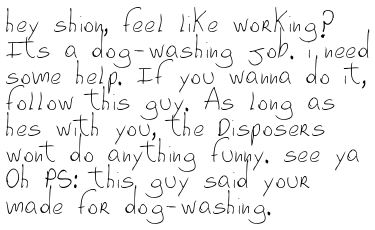
\includegraphics{Images/memo4.png}\\

"What's dog-washing?"

"It's just how it reads. You wash dogs― the ones that Inukashi lends out
for heating. They're the big, quiet ones with long fur. There must be
about twenty of them altogether. He gets customers sometimes that don't
pay because they complain the dogs are smelly or have fleas, so once a
week on a sunny day he takes them out for a wash. So what are you gonna
do?"

"I'll go, of course," Shion glowed. "He's asking me if I want to come
work. It's my first job. I actually have a job now."

"Will you stop gushing?" Nezumi said with a grimace. "Man, you really
are easy to please, aren't you?"

"Nezumi, should I take anything with me? Do you think I'll need soap?"

"You probably won't need anything. Just beware of men and women who
might pull you into alleyways, I guess. If that dog is with you, I don't
think you need to worry. I'll go with you partway."

"Speaking of which, I do want to see your workplace one day. And see you
on the stage."

"Don't get your hopes up."

The dog barked.

"Thank you," Shion told him. "Thanks to you, I've been able to get my
hands on my first job. I'm all yours, take me there."

The dog wagged its tail as Shion crouched down toward it, and licked him
under the chin.

"You're licking my wound for me? You're a nice boy."

"Dumbass, he only licked it because he smelled blood."

"I don't think so. He did it because he was concerned about me. But
whatever the reason, he's certainly nicer than you," Shion said wryly.

"Don't compare me with a mutt," Nezumi said sullenly. He looked
genuinely disgruntled. The way he stuck his lip out brought back a
fleeting image of his face four years ago. It somehow made Shion want to
laugh, and for some reason, made him feel nostalgic.

"What?" Nezumi said. "What're you grinning about?"

"Nothing," Shion said mildly. "Just noticing you've still got a childish
part left in you. It made me kind of happy."

"Huh?"

"Never mind. Alright, then," he said briskly, "lead the way." He petted
the dog lightly on the back. Picking up the cue, the dog bounded up the
stairs. Shion followed after it and exited the basement room.

The sun was bright in his eyes. I see― a day like this would be perfect
for washing dogs. He tilted his face up to the sky and breathed in
deeply.

It looked like Shion's figure was being sucked into the light. Whenever
Nezumi crawled out of his dark hole, the light always stabbed at his
eyes. He didn't like bright places. Places filled with light always
turned easily into areas of danger. He knew this well from experience.
He couldn't be like Shion and fully accept the light without hesitation.

Friends and enemies. Outside the wall, and inside the wall. Love and
hatred. Light and dark.

I told you, didn't I? They can never co-exist. I've told you so many
times, and you still don't seem to get it.

He swallowed a sigh that was halfway up his throat. The lump sank deep
down into his chest again.

As Nezumi was about to lock the door, a mouse came rubbing itself
against his foot.

"You're back." He scooped it up in his hand. The mouse seemed exhausted.
Its grape-coloured eyes were bleary.

"You've worked hard. Rest up." The mouse shook its head, and spat a
capsule onto Nezumi's palm. There was a light blue piece of paper
inside.

"A reply, huh." If it was, Shion would rejoice. Today must be a lucky
day for letters.

Just for an instant, a blackness flitted across his heart. A black
thing. It had no form― it was only dark. Uncertainty, a bad premonition.
A dull pain throbbed in the back of his head.

His ability to smell impending danger or calamity was something he had
had since birth. Thanks to this ability, he had been able to escape
numerous times, in some instances by a mere hair. The contents of this
capsule carried a bad smell. It smelled like the first step toward
something that would chase him into destruction....

He opened the capsule. The paper was scribbled with what looked like
Karan's handwriting.

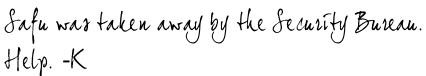
\includegraphics{Images/memo5.png}\\

The pain got worse. Nezumi screwed his eyes shut, and leaned heavily
against the door.

Safu― it was that girl.~Why was she―~wasn't she an elite? Just like
Shion... just like Shion... which means― she was taken in place of him?
The second scapegoat? But he didn't know for what reason. Why do they
need a sacrifice? Shion was framed as a murderer to cover up what the
parasite wasp did. They should only need one perpetrator. So why― why
did the authorities want another sacrifice? Why―

Either way, if that girl is the second sacrifice, she hasn't been taken
to the Security Bureau. She's headed for the Correctional Facility. A
mouse takes half a day to get back from No. 6. There's no more time.
She's probably been imprisoned in the Correctional Facility already.

Why were they eliminating so easily a Gifted Curriculum student that
they had measured, carefully selected, and spent considerable funds and
time to raise?

Why? Why― what was going on? What are they hiding? What's about to
happen?

Nezumi slowly brought himself upright.

He didn't know. It was a mystery. But now was not the time to be solving
puzzles. He had an important decision to make.

What to do with this?

If he showed this scribbled note to Shion, he would probably head right
for the Correctional Facility, without even knowing what kind of place
it was. He would go, with the single intention of rescuing Safu. A
sheltered simpleton of a little boy like him would never be able to let
a friend's death go unheeded. If he could prevent it, it was reason
enough for him to go diving head-first into a nest of venomous snakes.
He would willingly embark to his own death.

Or do I crush it?

It was very easy to do. This girl, Safu, had nothing to do with Nezumi.
She was a stranger. It wasn't any of his business what should happen to
her. He could leave things be, and it wouldn't matter. Nothing would
change.

But if Shion died, something within him would change greatly. He didn't
want to see Shion die. He would probably suffer. Not Shion, but he―
Nezumi― would suffer, from having to live and stand before Shion's
corpse. He would be experiencing the same suffering again, of being
broiled alive in hellfire.

You've gotta be kidding me. I've had enough of this already.

He didn't want to lose him. He didn't want to experience the remorse of
having been the one that lived.

I don't want to lose him? I would suffer?

He was clicking his tongue in frustration.

So this was what he had come to. He almost felt like curling up on the
ground.

He had rescued Shion from the hands of the Security Bureau to return the
debt that he owed him. That was it. He never wished to be attached to
him. Shion wasn't the only one― he had never wished to be attached or to
share his heart with any other person. Feelings for others were even
more dangerous than the light. He was not to share a connection with
anyone. Whether it be with a man or a woman, he was only to develop
relationships that could be severed easily.

Never open your heart to anyone. Don't believe in anyone but yourself.

The last words of the old woman. He was turning against them again.

I don't want to lose him. I would suffer.

Nezumi carefully folded Karan's memo again and stuffed it inside the
capsule.

He was used to loss, he was used to suffering. Wasn't he? Even if Shion
did die, perhaps he wouldn't moan in agony over his gaping loss. Even if
he did, perhaps it would only be for a short while.

He would be able to use his bed and shower freely. He wouldn't have to
worry about making enough soup. He wouldn't be pelted incessantly with
questions, or be spoken to. He would be released from having to look up
halfway through a book to lend an ear to the other's words, and to give
an answer while trying to restrain his irritation.

He would go back to his normal life. That was it. He should just pass
the memo, capsule and all, to Shion, and then turn his back on him.

On a whim, Nezumi opened his door again.

Before him was his room, filled with books and sparse furniture. The
basement chamber, surrounded by thick walls, was a nest that suited a
rat like him well.

The room looked barren and dark, and larger than usual. Its coldness,
darkness and vacant space seeped into his bones.

That was what being attached to someone meant. He would no longer be
able to live alone anymore. It was one of many artfully-set traps that
lurked at every corner of his life. And to this one, he had fallen
victim.

Have I still got a chance?

"Nezumi, what's wrong?" Shion called from the top of the stairs, the
entrance that led to ground-level. "The dog's pulling at me. Hurry and
come on up." His shadowy figure floated up against the glare of noon.

Have I still got a chance? Shion, will I still be able to live without
you? After some amount of suffering, would I be able to detach myself
from the trap you've become?

Would I be able to sever you?

"Nezumi?" The voice from above dropped apprehensively.

"Nothing― I'm coming." He closed the door. He heard the dog bark. There
was light. The rustle of a breeze.

Nezumi wrapped the superfibre cloth around his neck again, and ascended
the stairs step by step. He kept ascending to the ground above.

\protect\hypertarget{index_split_138.html}{}{}

\hypertarget{index_split_138.htmlux5cux23calibre_pb_142}{%
\subsection{Volume 2}\label{index_split_138.htmlux5cux23calibre_pb_142}}

Volume 2 (tankobon)

As you are reading this particular page of the story right now, what
sort of scene is unfolding around you?

What is happening with the wars, with starvation, with the world? Is the
killing still continuing? Is hatred still overflowing? Is despair still
brimming?

Do you believe in the word "hope"? I've always wanted to believe in
it―that the world could be mended, that people would be able to throw
their weapons aside. Someday.

Writing stories for young people is none other than to tell a tale of
hope―because there should be nothing born from despair.

That was how I've felt up until now, and obedient to that belief, I've
been weaving stories that tell of hope, but cavalierly.

"You don't know anything. You don't know what it's like to starve, to
shiver in the cold, to groan from a wound that's festered because it's
been left untreated too long; you don't know the suffering that follows
when that wound becomes infested with maggots, and you start rotting
alive; you don't know how it feels to watch someone die in front of you,
while there's nothing you can do to help them. You don't know a single
thing. You're just rattling off pretty words."

"You're just looking for an escape route. You're looking for a way to
avoid getting hurt."

"Words aren't things that you can toss around casually. You can't let
yourself be forced to say something, and just put up with it. But you
don't know that. So that's why I'm not going to trust you."

The numerous harsh words that Nezumi hurled at Shion were also blades
bared against me, and needles that stabbed my body.

Yes: I feel like I've lived thus far without knowing anything, nor
trying to know. I suffer no ailments; I never need to worry about food
for tomorrow; I live life without having to feel a smidgeon of fear from
being blasted by landmines or rocket bombs. I love my somewhat boring,
but peaceful life. And that's fine in itself. But when I peeled back a
bit of that peaceful life, I couldn't go without seeing that it was
actually very closely connected with foreign lands that seemed so
distant; with the war and starvation that people were suffering in those
lands.

Individuals are always connected to their nation, and the nation is
always connected to the rest of the world. It is impossible to cut them
apart. And I have finally realized that.

That was why I wanted to write this story, no matter what it took. Along
with a certain boy called Shion, I wanted to reach out and touch the
world. I wanted to write of a young and clumsy soul opening up his
physical body, and understanding the world through the pain and joy he
felt through it.

But to be honest, there were several times while writing when I thought
I would never be able to be like Shion. I couldn't face off with the
world as honestly as he. I couldn't yearn for another as earnestly. I
couldn't weave words as truthfully. And I was afraid of getting hurt. I
was always coming up with convenient excuses for myself. I couldn't beg
like he could.

At this point of having written up this story, for some reason I feel
something closer to defeat rather than fulfilment.

I'm sorry, here I go again, complaining. Those most unsteady in their
stance are the ones that talk the most, and make the most complaints.

Anyway, the story is still developing. I sincerely hope that you will be
able to enjoy it as Shion and Nezumi live, move, and weave their story
into existence.

I have no idea what will happen to these two, either. I'm not being mum
on purpose: I honestly can't predict what will happen.

But this is for certain: I do know that I don't want to leave Shion as
an idealist who is all talk; and I don't want to make Nezumi into a
terrorist of pure hatred. I would not want that to happen, no matter
what. So what do I need to do in order for it not to happen? What is
needed for them to survive, for them to avoid "becoming enemies", as
Nezumi once said? I know that I must think about this with a steady gaze
not on fantasy, but reality. And that must mean to focus the spotlight
on the ugliness of the nation-state, the frailty of human beings, my own
low-handedness, and never to avert that gaze.

And of course, in the end, I want to tell a tale of hope―not cavalierly,
with an agreeable smile on my face, using limp and lifeless words that
are merely pleasing to the ear. I want to speak with words I've invested
my own self into―I could mumble them, for what it's worth―but I want to
speak of hope, the kind I've grasped with my own hands. I want to become
that kind of writer.

I don't have the confidence I'll succeed. I already know very well how
powerless and incapable I am. But to me, it seems like there's still no
other way than to keep fighting alongside these young men.

I dedicate my heartfelt gratitude and hold in utmost admiration, Mr.
Yamakage Yoshikatsu of Kodansha's Editing Department, but at the same
time I want to complain to him, "It's so draining, this work." But I
know that he would probably―no, definitely―reply with, "You're being
indulgent. You're a professional. At least make sure you don't let
Nezumi and Shion laugh at you. Come on, straighten up."

Well, we've come to the end. My gratitude to the following people (no
complaints this time): Mr. Kageyama Toru, for creating the world of No.
6 more realistically, more fantastically, than anything my imagination
would have been able to create; and Mr. Kitamura Takashi, for giving No.
6 its unique glow and shadow through photos. Thank you.

February 2004

Asano Atsuko

Volume 2 (bunko)

To all of you who have read No. 6 \#2: first of all, I send you my
thanks from the bottom of my heart.

This time, I decided to lend the narrative point of view to Shion, and
write from his place in the interior of the citadel city of No. 6,
looking out into the outside world of the West Block.

What sort of image did that place reflect in your eyes and hearts,
readers? By continuing to write this story, I am continually faced by my
own hypocrisy, which can be emotionally stressing sometimes... no, all
the time. How can someone like me, who has never starved or froze, write
about people who live in the West Block?

If anything, it's arrogant and irresponsible; and for that reason I've
never liked to talk about this story, and if I force myself to open my
mouth, all that comes out is complaints and excuses. I'm sorry.

But still, to me, young men (and young women) of this age are
fascinating, and are figures that I have a profound attraction for. I so
badly want to know how they will live in this world, that instead of
learning from my mistakes, I arrogantly and irresponsibly continue to
write a story like No. 6. As I hold both joy and fear in my heart that
this book will be seen and read by more people in its form as a bunko, I
think I would like to live alongside these young men and women for just
a little longer.

Thank you very, very much for reading.

February 2007

Asano Atsuko
